\label{ch:compressible}

\section{Introduction}

\label{sec:eulermeth:intro}

The numerical methods we use for the Euler equations mirror those used
with advection in Ch.~\ref{ch:advection}.  The basic process is:
\begin{itemize}
\item Reconstruct the state variables to the interfaces.
\item Solve the Riemann problem (as described in
  \S~\ref{euler:sec:riemann}) and construct the fluxes through
  the interfaces.
\item Perform the conservative update on the state variables.
\end{itemize}
The Euler equations are much more complicated than linear
advection---we already saw this with the Riemann problem.  But we will
also see that in different parts of the algorithm we will use
conservative or primitive variables.  Additional physics can enter as
source terms, which we'll see how to add to both the interface states
and conservative update here.

%-----------------------------------------------------------------------------
\section{Reconstruction of interface states}

\label{sec:onedrecon}

We will solve the Euler equations using a high-order {\em Godunov
  method}---a finite volume method whereby the fluxes through the
interfaces are computed by solving the Riemann problem for our system.
The finite-volume update for our system appears as:
\begin{equation}
\Uc^{n+1}_i = \Uc^n_i + \frac{\Delta t}{\Delta x} \left ( \Fb_{i-\myhalf}^{n+\myhalf} - \Fb_{i+\myhalf}^{n+\myhalf} \right )
\end{equation}
This says that each of the conserved quantities in $\Uc$ change only due
to the flux of that quantity through the boundary of the cell.

Instead of approximating the flux itself on the interface, we find an
approximation to the state on the interface, $\Uc_{i-\myhalf}^{n+\myhalf}$ and
$\Uc_{i+\myhalf}^{n+\myhalf}$ and use this with the flux function to define the
flux through the interface:
\begin{align}
\Fb_{i-\myhalf}^{n+\myhalf} &= \Fb(\Uc_{i-\myhalf}^{n+\myhalf}) \\
\Fb_{i+\myhalf}^{n+\myhalf} &= \Fb(\Uc_{i+\myhalf}^{n+\myhalf})
\end{align}
To find this interface state, we predict left and right states at each
interface (centered in time), which are the input to the Riemann
solver.  The Riemann solver will then look at the characteristic wave
structure and determine the fluid state on the interface, which is
then used to compute the flux.  This is illustrated in
Figure~\ref{fig:riemann}.

Finally, although we use the conserved variables for the final update,
in constructing the interface states it is often easier to work with
the primitive variables.  These have a simpler characteristic
structure.  The interface states in terms of the primitive variables
can be converted into the interface states of the conserved variables
through a simple algebraic transformation,
\begin{equation}
\Uc_{i+\myhalf,L}^{n+\myhalf} = \Uc(\qb_{i+\myhalf,L}^{n+\myhalf})
\end{equation}

% figure made with figures/Euler/riemann-states.py
\begin{figure}[t]
\centering
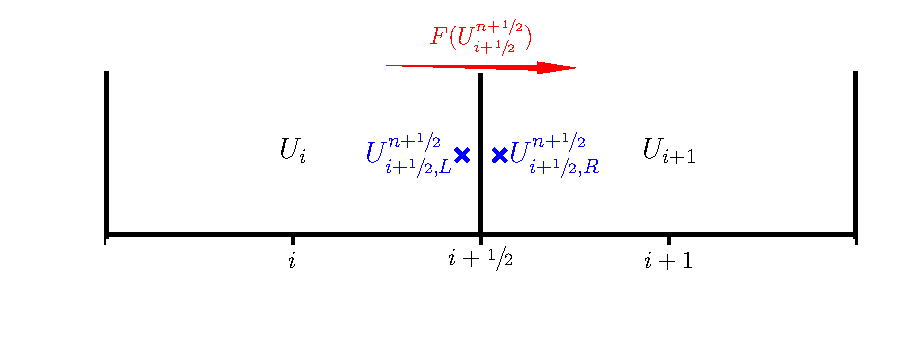
\includegraphics[width=\linewidth]{riemann_comp}
\caption[The left and right states for the Riemann
  problem]{\label{fig:riemann} The left and right states at interface
  $i+\myhalf$.  The arrow indicates the flux through the interface, as
  computed by the Riemann solver using these states as input.}
\end{figure}

As we saw with linear advection in \S~\ref{ch:adv:sndorder},
at the start of a timestep, each zones contains cell-averages.
Consider a cell average quantity, $\qb_i$.
Constructing the interface states requires reconstructing the
cell-average data as a continuous function, $\qb(x)$, defined for
each cell.  This polynomial is only {\em piecewise} continuous, since
each cell has its own $\qb(x)$.  Standard choices are piecewise constant,
\begin{equation}
\qb(x) = \qb_i
\end{equation}
piecewise linear,
\begin{equation}
\qb(x) = \qb_i + \frac{\Delta \qb_i}{\Delta x}(x - x_i)
\end{equation}
or piecewise parabolic,
\begin{equation}
\qb(x) = \boldsymbol{\alpha} (x - x_i)^2 + \boldsymbol{\beta} (x - x_i) + \boldsymbol{\gamma}
\end{equation}
where in each case, the average of $\qb(x)$ over the cell gives $\qb_i$.
Most of the complexity of the method is then figuring out the coefficients
of the polynomial.

Characteristic tracing is then done under this polynomial to see how
much of each characteristic quantity comes to the interface over the
timestep.  The jump in the primitive variables is projected into the
characteristic variables, and only jumps moving toward the interface
are included in our reconstruction.  We look at several methods below
that build off of these ideas below.

\subsection{Piecewise constant}

The simplest possible reconstruction of the data is piecewise constant.
This is what was done in the original Godunov method~\cite{godunov:1959}.  For the interface
marked by $i+\myhalf$, the left and right states on the interface are simply:
\begin{align}
\Uc_{i+\myhalf,L} &= \Uc_i \\
\Uc_{i+\myhalf,R} &= \Uc_{i+1}
\end{align}
This does not take into account in any way how the state $\Uc$ may be changing
through the cell.  As a result, it is first-order accurate in space, and since
no attempt was made to center it in time, it is first-order accurate in time.

\subsection{Piecewise linear}

For higher-order reconstruction, we first convert from the conserved
variables, $\Uc$, to the primitive variables, $\qb$.  These have a simpler
characteristic structure, making them easier to work with.  Here we
consider piecewise linear reconstruction---the cell average data is
approximated by a line with non-zero slope within each cell.
Figure~\ref{fig:plm} shows the piecewise linear reconstruction of some
data.


% figure made with figures/Euler/ppm.py
\begin{figure}[t]
\centering
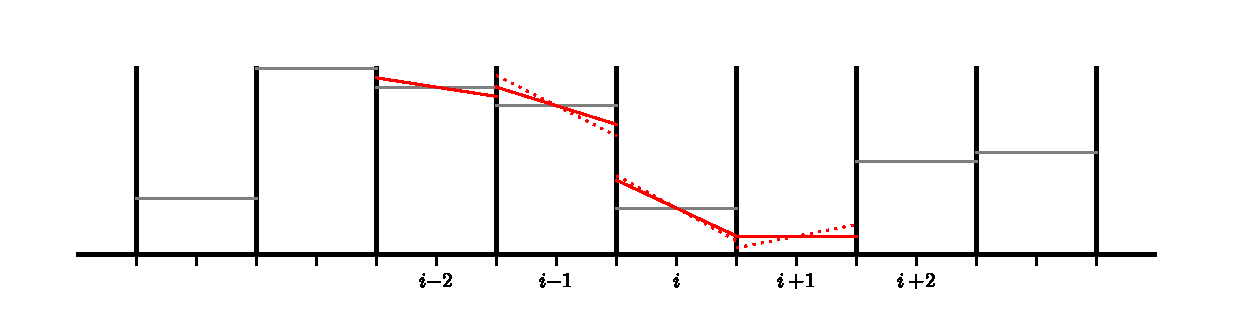
\includegraphics[width=\linewidth]{piecewise-linear}
\caption[Piecewise linear reconstruction of cell average
  data]{\label{fig:plm} Piecewise linear reconstruction of the cell
  averages.  The dotted line shows the unlimited center-difference
  slopes and the solid line shows the limited slopes.}
\end{figure}

Consider constructing the left state at the interface $i+\myhalf$ (see
Figure~\ref{fig:riemann}).  Just like for the advection equation, we
do a Taylor expansion through $\Delta x/2$ to bring us to the
interface, and $\Delta t/2$ to bring us to the midpoint in time.
Starting with $\qb_i$, the cell-centered primitive variable, expanding
to the right interface (to create the left state there) gives:
\begin{align}
\qb_{i+\myhalf,L}^{n+\myhalf} &= \qb_i^n +
    \left . \frac{\Delta x}{2} \frac{\partial \qb}{\partial x} \right |_i +
    \frac{\Delta t}{2} \underbrace{\left .\frac{\partial \qb}{\partial t} \right |_i}_{= -\Ab \partial \qb / \partial x} + \ldots \\
&= \qb_i^n + \frac{\Delta x}{2} \left . \frac{\partial \qb}{\partial x} \right |_i
          - \frac{\Delta t}{2} \left ( \Ab \frac{\partial \qb}{\partial x} \right )_i\\
&= \qb_i^n + \frac{1}{2} \left [ 1 - \frac{\Delta t}{\Delta x} \Ab_i \right ] \Delta \qb_i \label{eq:taylorstate}
\end{align}
where $\Delta \qb_i$ is the reconstructed slope of the primitive
variable in that cell (similar to how we compute it for the advection
equation).  We note that the terms truncated in the first line are
$O(\Delta x^2)$ and $O(\Delta t^2)$, so our method will be second-order
accurate in space and time.

As with the advection equation, we limit the slope such that no new minima
or maxima are introduced.  Any of the slope limiters used for linear advection
apply here as well.  We represent the limited slope as $\overline{\Delta \qb}_i$.

We can decompose $\Ab \Delta \qb$ in terms of the left and right
eigenvectors and sum over all the waves that move {\em toward} the
interface.  First, we recognize that $\Ab = R \Lambda L$ and recognizing
that the `$1$'
in Eq.~\ref{eq:taylorstate} is the identity, $I = LR$, we rewrite this
expression as:
\begin{equation}
\qb_{i+\myhalf,L}^{n+\myhalf} = \qb_i^n +
     \frac{1}{2} \left [ \Rb\Lb - \frac{\Delta t}{\Delta x} \Rb\Lambdab \Lb \right ]_i \overline{\Delta \qb}_i
\end{equation}
We see the common factor of $\Lb \Delta \qb$.  We now write this back in
component form.  Consider:
\begin{equation}
\renewcommand{\arraystretch}{1.5}
\Rb\Lambdab \Lb \overline{\Delta \qb} =
   \left ( \begin{array}{c:c:c}
             r_1^\evm & r_1^\evz & r_1^\evp \\
             r_2^\evm & r_2^\evz & r_2^\evp \\
             r_3^\evm & r_3^\evz & r_3^\evp \end{array} \right )
   \left ( \begin{array}{ccc}
             \lambda^\evm &              & \\
                          & \lambda^\evz & \\
                          &              & \lambda^\evp \end{array} \right )
   \left ( \begin{array}{ccc}
             l_1^\evm & l_2^\evm & l_3^\evm \\
             \hdashline
             l_1^\evz & l_2^\evz & l_3^\evz \\
             \hdashline
             l_1^\evp & l_2^\evp & l_3^\evp \end{array} \right )
   \left ( \begin{array}{c}
            \overline{\Delta \rho} \\
            \overline{\Delta u} \\
            \overline{\Delta p} \end{array} \right )
\renewcommand{\arraystretch}{1.0}
\end{equation}
Starting with $\Lb \overline{\Delta \qb}$, which is a vector with each component
the dot-product of a left eigenvalue with $\overline{\Delta \qb}$, we have
\begin{equation}
\renewcommand{\arraystretch}{1.5}
\Rb\Lambdab \Lb \overline{\Delta \qb} =
   \left ( \begin{array}{c:c:c}
             r_1^\evm & r_1^\evz & r_1^\evp \\
             r_2^\evm & r_2^\evz & r_2^\evp \\
             r_3^\evm & r_3^\evz & r_3^\evp \end{array} \right )
   \left ( \begin{array}{ccc}
             \lambda^\evm &              & \\
                          & \lambda^\evz & \\
                          &              & \lambda^\evp \end{array} \right )
   \left ( \begin{array}{c}
            \lb^\evm \cdot \overline{\Delta \qb} \\
            \lb^\evz \cdot \overline{\Delta \qb} \\
            \lb^\evp \cdot \overline{\Delta \qb} \end{array} \right )
\renewcommand{\arraystretch}{1.0}
\end{equation}
Next we see that multiplying this vector by $\Lambdab$ simply puts the
eigenvalue with its respective eigenvector in the resulting column vector:
\begin{equation}
\renewcommand{\arraystretch}{1.5}
\Rb\Lambdab \Lb \overline{\Delta \qb} =
   \left ( \begin{array}{c:c:c}
             r_1^\evm & r_1^\evz & r_1^\evp \\
             r_2^\evm & r_2^\evz & r_2^\evp \\
             r_3^\evm & r_3^\evz & r_3^\evp \end{array} \right )
   \left ( \begin{array}{c}
            \lambda^\evm \, \lb^\evm \cdot \overline{\Delta \qb} \\
            \lambda^\evz \, \lb^\evz \cdot \overline{\Delta \qb} \\
            \lambda^\evp \, \lb^\evp \cdot \overline{\Delta \qb} \end{array} \right )
\renewcommand{\arraystretch}{1.0}
\end{equation}
Finally, the last multiply results in a column vector:
\begin{equation}
\renewcommand{\arraystretch}{1.5}
R\Lambda L \overline{\Delta \qb} =
   \left ( \begin{array}{c}
            r_1^\evm \, \lambda^\evm \, \lb^\evm \cdot \overline{\Delta \qb} +
            r_1^\evz \, \lambda^\evz \, \lb^\evz \cdot \overline{\Delta \qb} +
            r_1^\evp \, \lambda^\evp \, \lb^\evp \cdot \overline{\Delta \qb} \\
%
            r_2^\evm \, \lambda^\evm \, \lb^\evm \cdot \overline{\Delta \qb} +
            r_2^\evz \, \lambda^\evz \, \lb^\evz \cdot \overline{\Delta \qb} +
            r_2^\evp \, \lambda^\evp \, \lb^\evp \cdot \overline{\Delta \qb} \\
%
            r_3^\evm \, \lambda^\evm \, \lb^\evm \cdot \overline{\Delta \qb} +
            r_3^\evz \, \lambda^\evz \, \lb^\evz \cdot \overline{\Delta \qb} +
            r_3^\evp \, \lambda^\evp \, \lb^\evp \cdot \overline{\Delta \qb} \\
   \end{array} \right )
\renewcommand{\arraystretch}{1.0}
\end{equation}
We can rewrite this compactly as:
\begin{equation}
\sum_\nu \lambda^{(\nu)} (\lb^{(\nu)} \cdot \overline{\Delta \qb}) \rb^{(\nu)}
\end{equation}
where we use $\nu$ to indicate which wave we are summing over.  A similar
expansion is used for $\Rb\Lb \overline{\Delta \qb}$.  In fact, any vector
can be decomposed in this fashion:
\begin{equation}
{\boldsymbol{\chi}} = {\bf I} {\boldsymbol{\chi}} = \Rb \Lb {\boldsymbol{\chi}} = 
   \sum_\nu (\lb^\enu \cdot {\boldsymbol{\chi}}) \rb^\enu
\end{equation}
And then it is easy to see that the above manipulations for $\Ab \Delta \qb$
can be expressed as:
\begin{equation}
\Ab \Delta \qb =  \Ab \sum_\nu (\lb^\enu \cdot \overline{\Delta \qb}) \rb^\enu = 
  \sum_\nu (\lb^\enu \cdot \overline{\Delta \qb}) \Ab \rb^\enu = 
  \sum_\nu (\lb^\enu \cdot \overline{\Delta \qb}) \lambda^\enu \rb^\enu
\end{equation}
where we used $\Ab \rb^\enu = \lambda^\enu \rb^\enu$.  The quantity $(\lb^\enu
\cdot \overline{\Delta \qb})$ that shows up here is the projection of
the vector $\overline{\Delta \qb}$ into the characteristic variable
carried by wave $\nu$.  This sum shows, as discussed earlier, that each wave
carries a jump in the characteristic variable, with the jump in the primitive
variables proportion to the right eigenvector, $\rb^\enu$.

The resulting vector
for the left state is:
\begin{equation}
\qb_{i+\myhalf,L}^{n+\myhalf} = \qb_i^n + \frac{1}{2} \sum_{\nu; \lambda^{(\nu)} \ge 0}
  \left [ 1 - \frac{\Delta t}{\Delta x} \lambda_i^{(\nu)} \right ] (\lb_i^{(\nu)} \cdot \overline{\Delta \qb}_i) \rb_i^{(\nu)}
\end{equation}
Note that we make a slight change here, and only include a term in the sum if
its wave is moving toward the interface ($\lambda^\enu \ge 0$).  The quantity
$\Delta t \lambda^\enu/\Delta x$ inside the brackets is simply the CFL
number for the wave $\nu$.

Starting with the data in the $i+1$ zone and expanding to the left, we can
find the right state on the $i+\myhalf$ interface:
\begin{equation}
\qb_{i+\myhalf,R}^{n+\myhalf} = \qb_{i+1}^n - \frac{1}{2} \sum_{\nu; \lambda^{(\nu)} \le 0}
  \left [ 1 + \frac{\Delta t}{\Delta x} \lambda_{i+1}^{(\nu)} \right ] (\lb_{i+1}^{(\nu)} \cdot \overline{\Delta \qb}_{i+1}) \rb_{i+1}^{(\nu)}
\end{equation}


A good discussion of this is in Miller \& Colella
\cite{millercolella:2002} (Eq.\ 85).  This expression is saying that
each wave carries a jump in $\rb^{(\nu)}$ and only those jumps moving
toward the interface contribute to our interface state.  This
restriction of only summing up the waves moving toward the interface
is sometimes called {\em characteristic tracing}.  This decomposition
in terms of the eigenvectors and eigenvalues is commonly called a {\em
  characteristic projection}.  In terms of an operator, $P$, it can be
expressed as:
\begin{equation}
P {\boldsymbol{\chi}} = \sum_\nu (\lb^{(\nu)} . {\boldsymbol{\chi}}) \rb^{(\nu)}
\end{equation}
\begin{exercise}[Characteristic projection]
{
Show that $P \qb = \qb$, using the eigenvectors corresponding to the primitive
 variable form of the Euler equations.}
\end{exercise}
In the literature, sometimes a `$>$' or `$<$' subscript on $P$ is used
to indicate the characteristic tracing.

We could stop here, but Colella \& Glaz~\cite{colellaglaz:1985}
(p.\ 278) argue that the act of decomposing $\Ab$ in terms of the left
and right eigenvectors is a linearization of the quasi-linear system,
and we should minimize the size of the quantities that are subjected
to this characteristic projection.  To accomplish this, they suggest
subtracting off a {\em reference state}.  Saltzman (Eq.\ 8) further
argues that since only jumps in the solution are used in constructing
the interface state, and that the characteristic decomposition simply adds
up all these jumps, we can subtract off the reference state and
project the result.  In other words, we can write:
\begin{equation}
\qb_{i+\myhalf,L}^{n+\myhalf} - \qb_\mathrm{ref} = \qb_i^n - \qb_\mathrm{ref} +
  \frac{1}{2} \left [ 1 - \frac{\Delta t}{\Delta x} \Ab_i \right ] \overline{\Delta \qb}_i
\label{eq:lin_decomp}
\end{equation}
Then we subject the RHS to the characteristic projection---this tells
us how much of the quantity $\qb_{i+\myhalf,L}^{n+\myhalf} - \qb_\mathrm{ref}$
reaches the interface.  Colella \& Glaz (p.\ 278) and Colella
(Eq.\ 2.11) suggest
\begin{equation}
\qb_\mathrm{ref} = \tilde{\qb}_{i,L} \equiv \qb_i^n +
   \frac{1}{2} \left [ 1 - \frac{\Delta t}{\Delta x}
 \max(\lambda_i^\evp, 0) \right ] \overline{\Delta \qb}_i \label{eq:qref}
\end{equation}
where $\lambda^\evp$ is the fastest eigenvalue, and thus will see
the largest portion of the linear profiles.  Physically, this
reference state represents the jump carried by the fastest wave
moving toward the interface.  Then,
\begin{equation}
\qb_{i+\myhalf,L}^{n+\myhalf} - \tilde{\qb}_{i,L} = \frac{1}{2} \frac{\Delta t}{\Delta x}
  \left [ \max(\lambda_i^\evp,0) - \Ab_i \right ] \overline{\Delta \qb}_i
\end{equation}
and projecting this RHS (see Colella \& Glaz Eq. 43; Miller \& Colella Eq. 87),
and isolating the interface state, we have
\begin{align}
\qb_{i+\myhalf,L}^{n+\myhalf} &= \tilde{\qb}_{i,L} + \frac{1}{2} \frac{\Delta t}{\Delta x}
       \sum_{\nu; \lambda^{(\nu)} \ge 0} \lb_i^{(\nu)} \cdot \left [ \max(\lambda_i^\evp,0) - \Ab_i \right ]
                                           \overline{\Delta \qb}_i \, \rb_i^{(\nu)} \\
                    &= \tilde{\qb}_{i,L} + \frac{1}{2} \frac{\Delta t}{\Delta x}
       \sum_{\nu; \lambda^{(\nu)} \ge 0} \left [ \max(\lambda_i^\evp,0) - \lambda_i^{(\nu)} \right ]
                                          (\lb_i^{(\nu)} \cdot \overline{\Delta \qb}_i) \, \rb_i^{(\nu)}
\end{align}
This is equivalent to the expression in Saltzman~\cite{saltzman:1994}
(p.\ 161, first column, second-to-last equation) and
Colella~\cite{colella:1990} (p.\ 191, the group of expressions at the
end)\footnote{Since the combination $\lb^\enu \cdot \Delta \qb$
  appears so frequently, some sources represent this as $\beta^\enu$
  and then write the interface states as a linear combination of the
  $\beta$'s.  Some variation in the literation, depending on whether $\rho$
  or $\tau = 1/\rho$ is used as a primitive variable}.  The corresponding
  state to the right of this interface is:
\begin{equation}
\qb_{i+\myhalf,R}^{n+\myhalf} = \tilde{\qb}_{i+1,R} + \frac{1}{2} \frac{\Delta t}{\Delta x}
       \sum_{\nu; \lambda^\enu \le 0}
       \left [ \min(\lambda_{i+1}^\evm,0) - \lambda_{i+1}^\enu \right ]
       (\lb_{i+1}^\enu \cdot \overline{\Delta \qb}_{i+1}) \, \rb_{i+1}^\enu
\end{equation}
where now the reference state captures the flow from the $i+1$ zone
moving to the {\em left} to this interface (hence the appearance of
$\lambda^\evm$, the leftmost eigenvalue):
\begin{equation}
\tilde{\qb}_{i+1,R} = \qb_{i+1} - \frac{1}{2} \left [ 1 + \frac{\Delta t}{\Delta x} \min(\lambda_{i+1}^\evm,0) \right ] \overline{\Delta \qb}_{i+1}
\end{equation}

Side note: the data in zone $i$ will be used to construct the right
state at $i-\myhalf$ (the left interface) and the left state at $i+\myhalf$
(the right interface) (see Figure~\ref{fig:states}).  For this reason,
codes usually compute the eigenvectors/eigenvalues for that zone and
then compute $\qb_{i-\myhalf,R}^{n+\myhalf}$ together with $\qb_{i+\myhalf,L}^{n+\myhalf}$
in a loop over the zone centers.

% figure made by figures/Euler/states.py
\begin{figure}
\centering
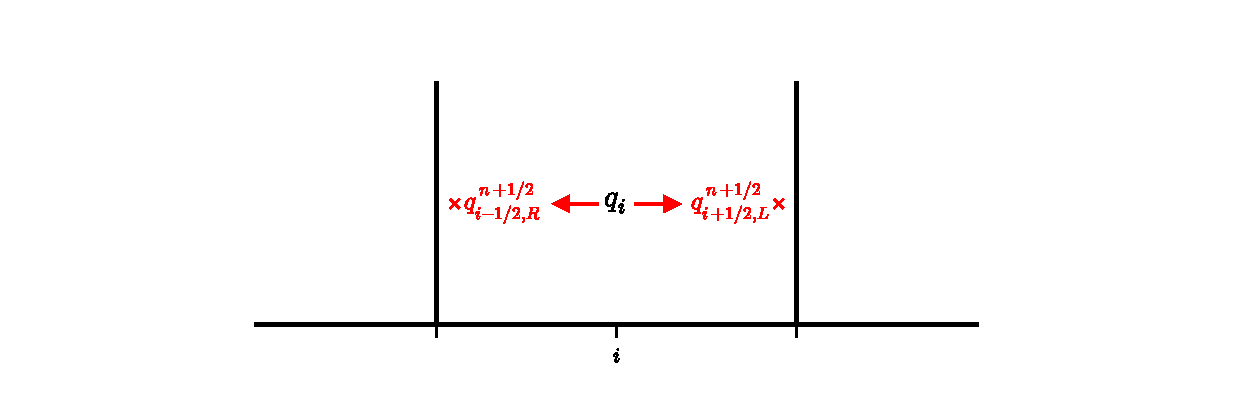
\includegraphics[width=3.5in]{states}
\caption[The two interface states derived from a cell-center quantity]{\label{fig:states} The two interface states that are constructed
using $\qb_i$ as the starting point.}
\end{figure}

\subsection{Piecewise parabolic}

\label{sec:hydro:ppm}

The piecewise parabolic method uses a parabolic reconstruction in each
cell.  This is more accurate than the linear reconstruction.
Figure~\ref{fig:ppm} shows the reconstructed parabolic profiles within
a few cells.  Since the original PPM
paper~\cite{colellawoodward:1984}, there have been many discussions of
the method, with many variations.  Here we focus on the presentation
by Miller \& Colella~\cite{millercolella:2002}, since that is the most
straightforward.  Note: even though a parabolic profile could be
third-order accurate, the temporal discretization and prediction in
this method is still only second-order.
%
% figure made by figures/Euler/ppm.py
\begin{figure}[t]
\centering
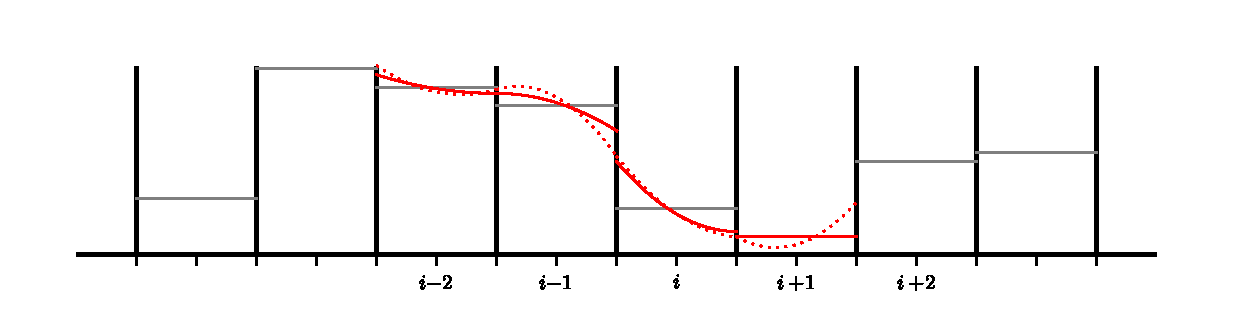
\includegraphics[width=\linewidth]{piecewise-parabolic}
\caption[Piecewise parabolic reconstruction of the cell
  averages]{\label{fig:ppm} Piecewise parabolic reconstruction of the
  cell averages.  The dotted line shows the unlimited parabolas---note
  how they touch at each interface, since the interface values come
  from the same interpolant initially.  The solid line shows the
  limited parabolas.}
\end{figure}


Miller \& Colella give an excellent description of how to take the
results for piecewise linear reconstruction and generalize it to the case of
PPM~\cite{colellawoodward:1984} (see Eqs.\ 88-90).  Starting with
Eq.~\ref{eq:lin_decomp}, we can write this (after the characteristic
projection) as
\begin{equation}
\qb_{i+\myhalf,L}^{n+\myhalf} = \tilde{\qb}_+ -
   \sum_{\nu;\lambda^{(\nu)}\ge 0} \lb_i^{(\nu)} \cdot \left \{
        \tilde{\qb}_+ - \left [ \qb_i^n +
            \frac{1}{2} \left ( 1 - \frac{\Delta t}{\Delta x} \lambda_i^{(\nu)} \right ) \overline{\Delta \qb}_i \right ]
       \right \} \rb_i^{(\nu)}
\end{equation}
Miller \& Colella rewrite the portion inside the $[\ldots]$
recognizing that (similar to M\&C Eq.\ 88, but for the $i+\myhalf,L$ interface):
\begin{equation}
  \qb_i^n + \frac{1}{2} \left (1 - \frac{\Delta t}{\Delta x} \lambda_i^{(\nu)} \right ) \overline{\Delta \qb}_i
  \approx \frac{1}{\lambda \Delta t} \int_{x_{i+\myhalf} - \lambda \Delta t}^{x_{i+\myhalf}}
           \qb(x) dx
\end{equation}
where $\qb(x)$ is the reconstructed functional form of $\qb$ in the zone.

\begin{exercise}[The average state reacting the interface]
{Show that this is exactly true for a linear reconstruction of $\qb(x)$, i.e.,
$\qb(x) = \qb_i + (\partial \qb/\partial x) (x - x_i)$.}
\end{exercise}

\noindent The integral on the right represents the average of $\qb$ that
can reach the right interface of the cell $i$ over timestep $\Delta
t$, moving at the wavespeed $\lambda$.  This suggests that we can
replace the linear reconstruction of $\qb$ with a parabolic one, and
keep our expressions for the interface states.

% figure made by figures/Euler/ppm-trace.py
\begin{figure}
\centering
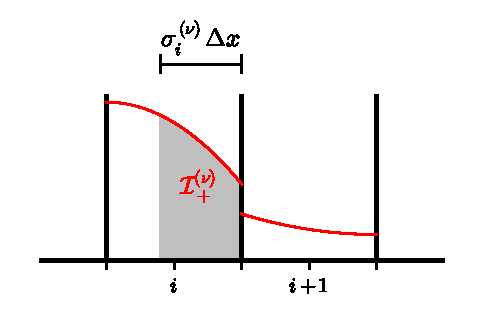
\includegraphics[width=3.5in]{ppm-trace}
\caption[Integration under the parabola profile for to an
  interface]{\label{fig:ppm_trace} Integration under the parabolic
  profile.  For each of the waves, $\sigma^\enu$ is the fraction of
  the cell that they cross in a timestep, and $\sigma^\enu \Delta x =
  \lambda^\enu \Delta t$ is the distance they can travel.  Here we are
  integrating under the parabola to the right interface of cell $i$ to
  define $\Ic_+^\enu$ (this is indicated by the shaded
  region).  The $\Ic_+^\enu$ carried by this wave will be
  added to those carried by the other waves to form the left state at
  interface $i+\myhalf$.}
\end{figure}

In particular, we define
\begin{equation}
\Ic_+^{(\nu)}(\qb_i) = \frac{1}{\sigma^{(\nu)} \Delta x} \int _{x_{i+\myhalf} - \sigma^{(\nu)} \Delta x}^{x_{i+\myhalf}} \qb(x) dx
\end{equation}
with $\sigma^{(\nu)} = |\lambda^{(\nu)}|\Delta t / \Delta x$ (see Almgren et
al. Eq. 31)  (see Figure~\ref{fig:ppm_trace}).  Then
\begin{equation}
\qb_{i+\myhalf,L}^{n+\myhalf} = \tilde{\qb}_+ -
   \sum_{\nu;\lambda^{(\nu)}\ge 0} \lb_i^{(\nu)} \cdot \left (
        \tilde{\qb}_+ - \Ic_+^{(\nu)}(\qb_i)
       \right ) \rb_i^{(\nu)}  \label{eq:ppmtrace}
\end{equation}
Miller \& Colella choose the reference state as
\begin{equation}
\tilde{\qb}_+ = \left \{ \begin{array}{cc}
       \Ic_+^{(+)}(\qb_i) & \mathrm{if~} u + c > 0 \\
       \qb_i                    & \mathrm{otherwise}
\end{array}
\right .
\end{equation}
where the superscript $(+)$ on $\Ic$ indicates that the
fastest eigenvalue ($\lambda^\evp = u + c$) is used.  This is similar in
spirit to Eq.~\ref{eq:qref}.  Note: in the original PPM paper, if the
wave is not approaching the interface, instead of using the
cell-average, $\qb_i$, they use the limit of the quadratic interpolant.
In contrast to the above, the Castro paper~\cite{almgren:2010} just
uses $\qb_i$ for the reference state regardless of whether the wave is
moving toward or away from the interface.  Note that if the system
were linear, then the choice of reference state would not matter.

To finish the reconstruction, we need to know the parabolic form
of $\qb(x)$.  Here, we do the reconstruction from the original PPM
paper:
\begin{equation}
\qb(x) = \qb_{-} + \xi(x) \left ( \Delta \qb + \qb_6 (1 - \xi(x) ) \right )
\end{equation}
with $\Delta \qb = \qb_+ - \qb_-$, and $\qb_-$, $\qb_+$ the values of the polynomial
on the left and right edges, respectively, of the current cell, and
\begin{equation}
\qb_6 \equiv 6 \left [ \qb_i - \frac{1}{2} (\qb_- + \qb_+) \right ]
\end{equation}
and
\begin{equation}
\xi(x) = \frac{x - x_{i-\myhalf}}{\Delta x}
\end{equation}

To complete the description, we need to determine the parameters of
the parabola.  The values of $\qb_-$ and $\qb_+$ are computed and limited
as described in the original PPM paper.  With this definition, we can
do the integral $\Ic_+$:
\begin{equation}
\Ic_+^{(\nu)}(\qb_i) = \qb_{+,i} - \frac{\sigma_i^{(\nu)}}{2}
   \left [ \Delta \qb_i - \qb_{6,i} \left ( 1 - \frac{2}{3} \sigma_i^{(\nu)} \right ) \right ]
\end{equation}
Figure~\ref{fig:ppm_trace} illustrates the process of integrating under
the parabolic profile.


\begin{exercise}[Conservative interpolation]
{Show that $\qb(x)$ is a conservative interpolant.  That is
\begin{equation}
\frac{1}{\Delta x} \int_{x_{i-\myhalf}}^{x_{i+\myhalf}} \qb(x) dx = \qb_i
\end{equation}
You can also see that the average over the left half of the zone is
$\qb_i -\frac{1}{4}\Delta \qb$ and the average over the right half of the
zone is $\qb_i + \frac{1}{4}\Delta \qb$.  This means that there are equal
areas between the integral and zone average on the left and right
sides of the zone.  This can be seen by looking at
Figure~\ref{fig:ppm}.  }
\end{exercise}

\begin{quote}
\noindent\makebox[\linewidth]{\rule{0.9\textwidth}{1pt}}
{\em Aside}:
Note that this characteristic projection of $\tilde{\qb}_+ -
\Ic_+^{(\nu)}$ is discussed in the original PPM paper in the
paragraph following their Eq.~3.5.  They do not keep things in this form
however, and instead explicitly multiply out the $l\cdot [\ldots] r$
terms to arrive at their Eq.~3.6.  For example, starting with
Eq.~\ref{eq:ppmtrace},
we can write the left velocity state as (leaving off the $i$
subscripts on the vectors):
\begin{equation}
u_{i+\myhalf,L}^{n+\myhalf} =
  \tilde{u}_+ - \sum_\nu \lb^{(\nu)} \cdot
      ( \tilde{\qb}_+ -  \Ic_+^{(\nu)}(\qb) )
    \underbrace{\rb^{(\nu)}}_{\begin{smallmatrix}\mathrm{only~the}\\ u~\mathrm{`slot'} \end{smallmatrix}}
\end{equation}
(where, as above, the $\sim$ indicates the reference state).
Here the $r$ eigenvector on the end is representative---we only pick
the row corresponding to $u$ in the $\qb$ vector (in our case, the
second row).

Putting in the eigenvectors and writing out the sum, we have:
\begin{align}
 u_{i+\myhalf,L}^{n+\myhalf} =
     \tilde{u}_+ &-
       \left ( \begin{array}{ccc}
                  0 & -\frac{\rho}{2c} & \frac{1}{2c^2} \end{array}
       \right )
    \left ( \begin{array}{c}
           \tilde{\rho}_+ - \Ic_+^\evm(\rho) \\
           \tilde{u}_+ - \Ic_+^\evm(u) \\
           \tilde{p}_+ - \Ic_+^\evm(p)
            \end{array} \right )
    {\color{mygray} \left ( \begin{array}{c}
           1  \\
           {\color{black} -c/\rho} \\
           c^2
    \end{array} \right ) } \nonumber \\
%
     &-\left ( \begin{array}{ccc}
                  1 & 0 & -\frac{1}{c^2} \end{array}
       \right )
    \left ( \begin{array}{c}
           \tilde{\rho}_+ - \Ic_+^\evz(\rho) \\
           \tilde{u}_+ - \Ic_+^\evz(u) \\
           \tilde{p}_+ - \Ic_+^\evz(p)
            \end{array} \right )
    {\color{mygray} \left ( \begin{array}{c}
           1  \\
           {\color{black} 0} \\
           0
    \end{array} \right ) } \nonumber \\
%
    &-\left ( \begin{array}{ccc}
                  0 & \frac{\rho}{2c} & \frac{1}{2c^2} \end{array}
       \right )
    \left ( \begin{array}{c}
           \tilde{\rho}_+ - \Ic_+^\evp(\rho) \\
           \tilde{u}_+ - \Ic_+^\evp(u) \\
           \tilde{p}_+ - \Ic_+^\evp(p)
            \end{array} \right )
    {\color{mygray} \left ( \begin{array}{c}
           1  \\
           {\color{black} c/\rho} \\
           c^2
    \end{array} \right ) }
%
\end{align}
Here again we show the entire right eigenvector for illustration, but
only the element that comes into play is drawn in black.  This shows
that the second term is $0$---the contact wave does not carry a jump
in velocity.  Multiplying out $\lb^{(\nu)} \cdot (\tilde{\qb}_+ -
\Ic_+^{(\nu)})$ we have:
\begin{align}
u_{i+\myhalf,L}^{n+\myhalf} =
   \tilde{u}_+
  &- \frac{1}{2} \left [
      (\tilde{u}_+ - \Ic_+^\evm(u) ) -
       \frac{\tilde{p}_+ - \Ic_+^\evm(p)}{C} \right ] \nonumber \\
  &- \frac{1}{2} \left [
      (\tilde{u}_+ - \Ic_+^\evp(u) ) +
       \frac{\tilde{p}_+ - \Ic_+^\evp(p)}{C} \right ]
\label{eq:ufull}
\end{align}
where $C$ is the Lagrangian sound speed ($C = \sqrt{\gamma p \rho}$).
Defining
\begin{align}
\beta^\evp &= - \frac{1}{2C}
  \left [
      (\tilde{u}_+ - \Ic_+^\evp(u) ) +
       \frac{\tilde{p}_+ - \Ic_+^\evp(p)}{C} \right ] \\
%
\beta^\evm &= + \frac{1}{2C}
  \left [
      (\tilde{u}_+ - \Ic_+^\evm(u) ) -
       \frac{\tilde{p}_+ - \Ic_+^\evm(p)}{C} \right ]
\end{align}
we can write our left state as:
\begin{equation}
u_{i+\myhalf,L}^{n+\myhalf} =
   \tilde{u}_+ + C ( \beta^\evp - \beta^\evm)
\end{equation}
This is Eqs.~3.6 and 3.7 in the PPM paper.  Note that in their
construction appears to use the reference state in defining the
Lagrangian sound speed (in their $\beta$ expressions is written as
$\tilde{C}$).  This may follow from the comment before Eq.~3.6,
``modified slightly for the present application''.  Similarly,
the expressions for $\rho_L$ and $p_L$ can be written out. \\
\noindent\makebox[\linewidth]{\rule{0.9\textwidth}{1pt}}
\end{quote}

Similar expressions can be derived for the right state at the left interface
of the zone ($\qb_{i-\myhalf,R}^{n+\myhalf}$).  Here, the integral under the parabolic
reconstruction is done over the region of each wave that can reach the left
interface over our timestep:
\begin{equation}
\Ic_-^{(\nu)}(\qb) = \frac{1}{\sigma^{(\nu)} \Delta x}
  \int_{x_{i-\myhalf}}^{x_{i-\myhalf} + \sigma^{(\nu)} \Delta x} \qb(x) dx
\end{equation}
The right state at $i-\myhalf$ using zone $i$ data is:
\begin{equation}
\qb_{i-\myhalf,R}^{n+\myhalf} = \tilde{\qb}_- - \sum_{\nu; \lambda_\nu \le 0}
   \lb_i^{(\nu)} \cdot \left ( \tilde{\qb}_- - \Ic_-^{(\nu)}(\qb_i) \right ) \rb_i^{(\nu)}
\end{equation}
where the reference state is now:
\begin{equation}
\tilde{\qb}_- = \left \{ \begin{array}{cc}
   \Ic_-^{(-)}(\qb_i) & \mathrm{if~} u - c < 0 \\
    \qb_i                   & \mathrm{otherwise}
\end{array} \right .
\end{equation}
where the $(-)$ superscript on $\Ic$ indicates that the most
negative eigenvalue $(\lambda^- = u - c)$ is used.  The integral
$\Ic_-^{(\nu)}(\qb)$ can be computed analytically by
substituting in the parabolic interpolant, giving:
\begin{equation}
\Ic_-^{(\nu)}(\qb_i) = \qb_{-,i} + \frac{\sigma_i^{(\nu)}}{2}
   \left [ \Delta \qb_i + \qb_{6,i} \left ( 1 - \frac{2}{3} \sigma_i^{(\nu)} \right ) \right ]
\end{equation}
This is equivalent to Eq.~31b in the Castro paper.

\subsubsection{New PPM limiters}

Recent work \cite{colellasekora} has formulated improved limiters for
PPM that do not clip the profiles at extrema.  This only changes the
limiting process in defining $\qb_+$ and $\qb_-$, and does not affect the
subsequent parts of the algorithm.


\subsection{Flattening and contact steepening}

  Shocks are self-steepening (this is how we
  detect them in the Riemann solver---we look for converging characteristics).
  This can cause trouble with the methods here, because the shocks may become
  too steep.

  Flattening is a procedure to add additional dissipation at shocks,
  to ensure that they are smeared out over $\sim 2$ zones.  The
  flattening procedure is a multi-dimensional operation that looks at
  the pressure and velocity profiles and returns a coefficient, $\chi
  \in [0,1]$ that multiplies the limited slopes.  The convention most
  sources use is that $\chi = 1$ means no flattening (the slopes are
  unaltered), while $\chi = 0$ means complete flattening---the slopes
  are zeroed, dropping us to a first-order method.
  See for example in Saltzman~\cite{saltzman:1994}.  Once the flattening
  coefficient is determined, the interface state is blended with the
  cell-centered value via:
  \begin{equation}
  \qb_{i+\myhalf,\{L,R\}}^{n+\myhalf} \leftarrow (1 - \chi) \qb_i + \chi \qb_{i+\myhalf,\{L,R\}}^{n+\myhalf}
  \end{equation}

  Note that the flattening algorithm increases the stencil size of
  piecewise-linear and piecewise-parabolic reconstruction to 4 ghost cells
  on each side.  This is because the flattening procedure itself looks
  at the pressure 2 zones away, and we need to construct the flattening
  coefficient in both the first ghost cell (since we need the interface
  values there) and the second ghost cell (since the flattening procedure
  looks at the coefficients in its immediate upwinded neighbor).

  In contrast to shocks, contact waves
  do not steepen (they are associated with the middle characteristic
  wave, and the velocity does not change across that, meaning there
  cannot be any convergence).  The original PPM
  paper advocates a contact steepening method to artificially steepen
  contact waves.  While it shows good results in 1-d, it can be
  problematic in multi-dimensions.

  Overall, the community seems split over whether this term should be
  used.  Many people advocate that if you reach a situation where you
  think contact steepening may be necessary, it is more likely that
  the issue is that you do not have enough resolution.


\subsection{Limiting on characteristic variables}

Some authors (see for example, \cite{athena} Eqs.~37, 38) advocate
limiting on the characteristic variables rather than the primitive
variables.  The characteristic slopes for the quantity carried by the
wave $\nu$ can be found from the primitive variables
as: 
%
\begin{equation} 
\Delta w^{(\nu)} = \lb^{(\nu)} \cdot \Delta \qb 
\end{equation} 
%
any limiting would then be done to $\Delta w^{(\nu)}$ and the limited
primitive variables would be recovered as:
\begin{equation}
  \overline{\Delta \qb} = \sum_\nu \overline{\Delta w}^{(\nu)}
  \rb^{(\nu)} 
\end{equation} 
(here we use an overline to indicate limiting).

This is attractive because it is more in the spirit of the linear
advection equation and the formalism that was developed there.  A
potential downside is that when you limit on the characteristic
variables and convert back to the primitive, the primitive variables
may now fall outside of valid physical ranges (for example, negative
density).



%-----------------------------------------------------------------------------
\section{Riemann solvers}


Once the interface states are created, the Riemann solver is called.  This
returns the solution at the interface:
\begin{equation}
\qb_{i+\myhalf}^{n+\myhalf} = \mathcal{R}(\qb_{i+\myhalf,L}^{n+\myhalf}, \qb_{i+\myhalf,R}^{n+\myhalf})
\end{equation}

As discussed in \S~\ref{Euler:riemann:solution}, we need to determine
which state is on our interface to compute the fluxes through the
interface.  The full solution of the Riemann problem can be quite expensive,
so in practice, approximate Riemann solvers are used to speed
the computation.  Different Riemann solvers
will have different approximations for finding the speeds of the left,
center, and right wave, and evaluating the star state.  In the `star'
region, only $\rho$ jumps across the middle (contact) wave, the
pressure and velocity are constant across that wave (see $\rb^\evz$).
We determine the state in the star region ($\rho_l^*, \rho_r^*, u^*,
p^*$) by using the jump conditions for the Euler equations or the
Riemann invariants, as shown in \S~\ref{Euler:riemann:starstate}.
Some approximate Riemann solvers assume that both waves are shocks or
both are rarefactions, aimplying the form of the equation that
must be solved to find $p_\star$.

Two-shock solvers, like the one in \cite{colellaglaz:1985} are quite
common in astrophyiscs.  Figure~\ref{fig:euler:riemann-2shock-curve}
shows the Hugoniot curves for the Sod problem under the 2-shock
assumption---they are quite close to those for the true solution.  To
further save on cost, approximate Riemann solvers for general
equations of state often include additional thermodynamic information
at the interfaces that overconstrains the system, but can remove the
need to call an expensive equation of state routine in solving for the
star state.


\begin{figure}[t]
\centering
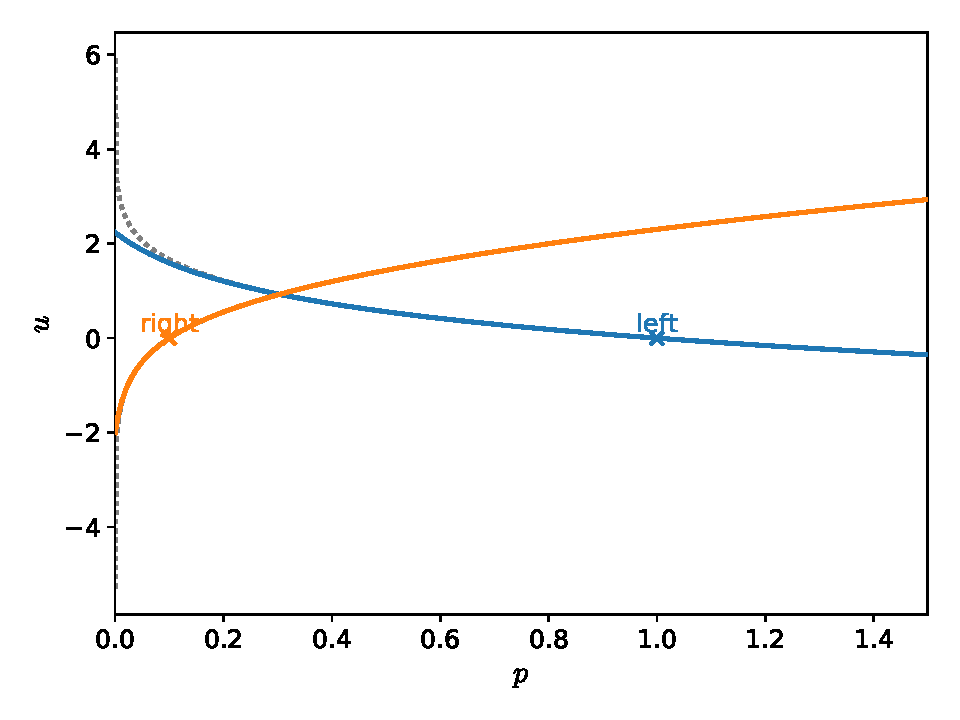
\includegraphics[width=0.9\linewidth]{riemann-2shock-sod-phase}
\caption[The approximate (2-shock) Hugoniot curves corresponding to
  the Sod problem]{\label{fig:euler:riemann-2shock-curve} The
  approximate Hugoniot curves under the 2-shock approximation
  corresponding to the Sod problem.  Also shown as the gray dotted
  line is the exact Hugoniot curves (compare to
  Figure~\ref{fig:euler:riemann-curve}).  We see that the 2-shock
  approximation does a reasonable job near the intersection and only
  diverges significantly for small $p$ (which is where the solution
  should really be a
  rarefaction).\\ 
  \hydroexdoit{\href{https://github.com/zingale/hydro_examples/blob/master/compressible/riemann-2shock.py}{riemann-2shock.py}}}
\end{figure}

An additional approximation concerns rarefactions.  Recall that a
rarefaction involves diverging flow---it spreads out with time.
Special consideration needs to be taken if the rarefaction wave spans
the interface (a {\em transonic rarefaction},
\S~\ref{Euler:riemann:solution}).  In this case, most approximate
Riemann solvers simply linearly interpolate between the left or right
state and the appropriate star state instead of solving for the
structure inside the rarefaction.

With this approximate state, the fluxes are computed as:
\begin{equation}
\renewcommand{\arraystretch}{1.5}
\Fb_{i+\myhalf}^{n+\myhalf} = \left ( \begin{array}{c}
                             \rho_{i+\myhalf}^{n+\myhalf} u_{i+\myhalf}^{n+\myhalf} \\
                             \rho_{i+\myhalf}^{n+\myhalf} (u_{i+\myhalf}^{n+\myhalf})^2 + p_{i+\myhalf}^{n+\myhalf} \\
                             u_{i+\myhalf}^{n+\myhalf} p_{i+\myhalf}^{n+\myhalf} / (\gamma - 1)  +
                             \frac{1}{2} \rho_{i+\myhalf}^{n+\myhalf} (u_{i+\myhalf}^{n+\myhalf})^3 +
                             u_{i+\myhalf}^{n+\myhalf} p_{i+\myhalf}^{n+\myhalf}
                            \end{array} \right )
\renewcommand{\arraystretch}{1.0}
\end{equation}

A different class of approximate Riemann solvers (the HLL family)
approximate the fluxes directly instead of approximating the state
first.  These require estimates of the wave speeds, and care must be
taken to ensure those estimates are valid for a general equation of
state.  These wave speeds are then used together with the
Rankine-Hugoniot jump conditions to give the fluxes.


%-----------------------------------------------------------------------------
\section{Conservative update}

Once we have the fluxes, the conservative update is done as
\begin{equation}
\Uc^{n+1}_i = \Uc^n_i + \frac{\Delta t}{\Delta x} 
   \left ( \Fb_{i-\myhalf}^{n+\myhalf} - \Fb_{i+\myhalf}^{n+\myhalf} \right )
\end{equation}
The timestep, $\Delta t$ is determined by the time it takes for the
fastest wave to cross a single zone:
\begin{equation}
\Delta t < \min_d \left \{ \frac{\Delta x}{|\Ub \cdot {\bf e}_d| + c}\right \}
\end{equation}
(This is the limit for the CTU unsplit scheme here, but see the discussion
in \S~\ref{sec:adv:timestep}).

Often simulation codes will further restrict the timestep.  Commonly
used restrictions for pure hydrodynamics include a limit on the factor
by which a timestep can grow from one step to the next (a typical
value is $1.2$), and an initial scaling, say of 1/10, for the first
timestep.  Together, these will force the code to take a few initial
steps before working up to the CFL limit.

\subsection{Artificial viscosity}

Colella and Woodward argue that behind slow-moving shocks these
methods can have oscillations.  The fix they propose is to use some
artificial viscosity---this is additional dissipation that kicks in at
shocks.  (They argue that flattening alone is not enough).

We use a multidimensional analog of their artificial viscosity
(\cite{colellawoodward:1984}, Eq.\ 4.5) which modifies the fluxes.  By
design, it only kicks in for converging flows, such that you would
find around a shock.


%-----------------------------------------------------------------------------
\section{Boundary conditions}

Boundary conditions are implemented through ghost cells.  The following
are the most commonly used boundary conditions.  For the expressions
below, we use the subscript $\mathrm{lo}$ to denote the spatial index
of the first valid zone in the domain (just inside the left boundary).

\begin{itemize}

\item {\em Outflow}: the idea here is that the flow should gracefully
  leave the domain.  The simplest form is to simply give all variables
  a zero-gradient:
  \begin{equation}
  \left ( \begin{array}{c} \rho_{\mathrm{lo-1},j} \\
                           (\rho u)_{\mathrm{lo-1},j} \\
                           (\rho v)_{\mathrm{lo-1},j} \\
                           (\rho E)_{\mathrm{lo-1},j} \end{array} \right ) =
  \left ( \begin{array}{c} \rho_{\mathrm{lo},j} \\
                           (\rho u)_{\mathrm{lo},j} \\
                           (\rho v)_{\mathrm{lo},j} \\
                           (\rho E)_{\mathrm{lo},j} \end{array} \right )
  \end{equation}

  Note that these boundaries are not perfect.  At the boundary, one
  (or more) of the waves from the Riemann problem can still enter
  the domain.  Only for supersonic flow, do all waves point outward.


\item {\em Reflect}: this is appropriate at a solid wall or symmetry
  plane.  All variables are reflected across the boundary, with the
  normal velocity given the opposite sign.  At the $x$-boundary, the
  first ghost cell is:
  \begin{equation}
  \left ( \begin{array}{c} \rho_{\mathrm{lo-1},j} \\
                           (\rho u)_{\mathrm{lo-1},j} \\
                           (\rho v)_{\mathrm{lo-1},j} \\
                           (\rho E)_{\mathrm{lo-1},j} \end{array} \right ) =
  \left ( \begin{array}{c} \rho_{\mathrm{lo},j} \\
                           -(\rho u)_{\mathrm{lo},j} \\
                           (\rho v)_{\mathrm{lo},j} \\
                           (\rho E)_{\mathrm{lo},j} \end{array} \right )
  \end{equation}
  The next is:
  \begin{equation}
  \left ( \begin{array}{c} \rho_{\mathrm{lo-2},j} \\
                           (\rho u)_{\mathrm{lo-2},j} \\
                           (\rho v)_{\mathrm{lo-2},j} \\
                           (\rho E)_{\mathrm{lo-2},j} \end{array} \right ) =
  \left ( \begin{array}{c} \rho_{\mathrm{lo+1},j} \\
                           -(\rho u)_{\mathrm{lo+1},j} \\
                           (\rho v)_{\mathrm{lo+1},j} \\
                           (\rho E)_{\mathrm{lo+1},j} \end{array} \right )
  \end{equation}
  and so on $\ldots$


  \item {\em Inflow}: inflow boundary conditions specify the state
    directly on the boundary.  Technically, this state is on the
    boundary itself, not the cell-center.  This can be accounted for
    by modifying the stencils used in the reconstruction near inflow
    boundaries.

  \item {\em Hydrostatic}: a hydrostatic boundary can be used at the
    base of an atmosphere to provide the pressure support necessary to
    hold up the atmosphere against gravity while still letting
    acoustic waves pass through.  An example of this is described
    in \cite{hse}.

\end{itemize}


%-----------------------------------------------------------------------------
\section{Multidimensional problems}

The multidimensional case is very similar to the multidimensional
advection problem.  Our system of equations is now:
\begin{equation}
\Uc_t + [\Fb^{(x)}(\Uc)]_x + [\Fb^{(y)}(\Uc)]_y = 0
\end{equation}
with
\begin{equation}
\Uc = \left ( \begin{array}{c} \rho \\ \rho u \\ \rho v \\ \rho E \end{array} \right )
%
\qquad
%
\Fb^{(x)}(\Uc) = \left ( \begin{array}{c} \rho u \\ \rho uu + p \\ \rho v u \\ \rho u E + up \end{array} \right )
%
\qquad
\Fb^{(y)}(\Uc) = \left ( \begin{array}{c} \rho v \\ \rho vu     \\ \rho v v + p \\ \rho v E + vp \end{array} \right )
\end{equation}

We note that there is no transformation that can convert the multidimensional
system into characteristic variables, since we cannot simultaneously
diagonalize the Jacobians corresponding to $\Fb^{(x)}$ and $\Fb^{(y)}$.  Related
to this is that when limiting, we limit one-dimensional slopes instead of
doing a full multidimensional reconstruction and limiting (see \cite{BDS}
for a multidimensional limiting procedure for linear advection.  For
the Euler equations, since we cannot write the multidimensional system
in a characteristic form, we cannot use this type of method).

For a directionally-unsplit discretization, we predict the
cell-centered quantities to the edges by Taylor expanding the
conservative state, $\Uc$, in space and time.  Now, when replacing the
time derivative ($\partial \Uc/\partial t$) with the divergence of the
fluxes, we gain a transverse flux derivative term.  For example,
predicting to the upper $x$ edge of zone $i,j$, we have:
\begin{align}
\Uc_{i+\myhalf,j,L}^{n+\myhalf} &= \Uc_{i,j}^n + \frac{\Delta x}{2} \frac{\partial \Uc}{\partial x}
                            + \frac{\Delta t}{2} \frac{\partial \Uc}{\partial t} + \ldots \\
&= \Uc_{i,j}^n + \frac{\Delta x}{2} \frac{\partial \Uc}{\partial x}
                            - \frac{\Delta t}{2} \frac{\partial \Fb^{(x)}}{\partial x}
                            - \frac{\Delta t}{2} \frac{\partial \Fb^{(y)}}{\partial y} \\
&= \Uc_{i,j}^n + \frac{1}{2} \left [ 1 - \frac{\Delta t}{\Delta x} \Ab^{(x)}(\Uc) \right ] \Delta \Uc
                            - \frac{\Delta t}{2} \frac{\partial \Fb^{(y)}}{\partial y} \label{eq:Utaylorstate}
\end{align}
where $\Ab^{(x)}(\Uc) \equiv \partial \Fb^{(x)} / \partial \Uc$.  We decompose
this into a {\em normal state} and a {\em transverse flux difference}.
Adopting the notation from Colella (1990), we use $\hat{\Uc}$ to denote
the normal state:
\begin{align}
\hat{\Uc}_{i+\myhalf,j,L}^{n+\myhalf} &\equiv \Uc_{i,j}^n
      + \frac{1}{2} \left [ 1 - \frac{\Delta t}{\Delta x} \Ab^{(x)}(\Uc) \right ] \Delta \Uc \\
\Uc_{i+\myhalf,j,L}^{n+\myhalf} &= \hat{\Uc}_{i+\myhalf,j,L}^{n+\myhalf}
                            - \frac{\Delta t}{2} \frac{\partial \Fb^{(y)}}{\partial y}  \label{eq:fullleftstate}
\end{align}

The primitive variable form for this system is
\begin{equation}
\qb_t + \Ab^{(x)}(\qb) \qb_x + \Ab^{(y)}(\qb) \qb_y = 0
\end{equation}
where
\begin{equation}
\qb = \left ( \begin{array}{c} \rho \\ u \\ v \\ p \end{array} \right )
%
\qquad
\Ab^{(x)}(\qb) = \left ( \begin{array}{cccc} u  & \rho     & 0 &  0 \\
                                         0  &  u       & 0 &  1/\rho \\
                                         0  &  0       & u &  0 \\
                                         0  & \gamma p & 0 &  u \end{array} \right )
\qquad
\Ab^{(y)}(\qb) = \left ( \begin{array}{cccc} v  & 0 & \rho &  0 \\
                                         0  & v & 0    &  0 \\
                                         0  & 0 & v    &  1/\rho \\
                                         0  & 0 & \gamma p & v \end{array} \right )
\end{equation}
There are now 4 eigenvalues.  For $\Ab^{(x)}(\qb)$, they are $u-c$, $u$,
$u$, $u+c$.  If we just look at the system for the $x$ evolution, we
see that the transverse velocity (in this case, $v$) just advects with
velocity $u$, corresponding to the additional eigenvalue.
\begin{exercise}[Eigenvectors for the 2-d Euler equations]
{
Derive the form of $\Ab^{(x)}(\qb)$ and $\Ab^{(y)}(\qb)$ and find their left and right eigenvectors.}
\end{exercise}

We note here that $\hat{\Uc}_{i+\myhalf,j,L}^{n+\myhalf}$ is essentially
one-dimensional, since only the $x$-fluxes are involved (through
$\Ab^{(x)}(\Uc)$).  This means that we can compute this term using the
one-dimensional techniques developed in \S~\ref{sec:onedrecon}.  In
particular, Colella (1990) suggest that we switch to primitive variables
and compute this as:
\begin{equation}
\hat{\Uc}_{i+\myhalf,j,L}^{n+\myhalf} = \Uc(\hat{\qb}_{i+\myhalf,j,L}^{n+\myhalf})
\end{equation}
Similarly, we consider the system projected along the $y$-direction to
define the normal states on the $y$-edges, again using the one-dimensional
reconstruction on the primitive variables from \S~\ref{sec:onedrecon}:
\begin{equation}
\hat{\Uc}_{i,j+\myhalf,L}^{n+\myhalf} = \Uc(\hat{\qb}_{i,j+\myhalf,L}^{n+\myhalf})
\end{equation}

To compute the full interface state (Eq.~\ref{eq:fullleftstate}), we
need to include the transverse term.
Colella (1990) gives two different procedures for evaluating the
transverse fluxes.  The first is to simply use the cell-centered
$\Uc_{i,j}$ (Colella 1990,
Eq. 2.13); the second is to use the reconstructed normal states (the
$\hat{\Uc}$'s) (Eq. 2.15).  In both cases, we need to solve a {\em
  transverse Riemann problem} to find the true state on the transverse
interface.  This latter approach is what we prefer.  In particular,
for computing the full $x$-interface left state, $\Uc_{i+\myhalf,j,L}^{n+\myhalf}$, we need the
transverse ($y$) states, which we define as
\begin{align}
\Uc^T_{i,j+\myhalf} &= \mathcal{R}(\hat{\Uc}^{n+\myhalf}_{i,j+\myhalf,L},
                            \hat{\Uc}^{n+\myhalf}_{i,j+\myhalf,R}) \\
\Uc^T_{i,j-\myhalf} &= \mathcal{R}(\hat{\Uc}^{n+\myhalf}_{i,j-\myhalf,L},
                            \hat{\Uc}^{n+\myhalf}_{i,j-\myhalf,R})
\end{align}

Taken together, the full interface state is now:
\begin{equation}
\Uc_{i+\myhalf,j,L}^{n+\myhalf} = \Uc(\hat{\qb}_{i+\myhalf,j,L}^{n+\myhalf})
   - \frac{\Delta t}{2} \frac{\Fb^{(y)}(\Uc^T_{i,j+\myhalf}) - \Fb^{(y)}(\Uc^T_{i,j-\myhalf})}{\Delta y}
\end{equation}

The right state at the $i+\myhalf$ interface can be similarly computed (starting with the
data in zone $i+1,j$ and expanding to the left) as:
\begin{equation}
\Uc_{i+\myhalf,j,R}^{n+\myhalf} = \Uc(\hat{\qb}_{i+\myhalf,j,R}^{n+\myhalf})
   - \frac{\Delta t}{2} \frac{\Fb^{(y)}(\Uc^T_{i+1,j+\myhalf}) - \Fb^{(y)}(\Uc^T_{i+1,j-\myhalf})}{\Delta y}
\end{equation}
Note the indices on the transverse states---they are now to the right of the interface (since
we are dealing with the right state).

We then find the $x$-interface state by solving the Riemann problem
normal to our interface:
\begin{equation}
\Uc_{i+\myhalf,j}^{n+\myhalf} = \mathcal{R}(\Uc_{i+\myhalf,j,L}^{n+\myhalf}, \Uc_{i+\myhalf,j,R}^{n+\myhalf})
\end{equation}
Therefore, construction of the interface states now requires two
Riemann solves: a transverse and normal one.  The fluxes are then evaluated as:
\begin{equation}
\Fb^{(x),n+\myhalf}_{i+\myhalf,j} = \Fb^{(x)}(\Uc_{i+\myhalf,j}^{n+\myhalf})
\end{equation}
Note, for multi-dimensional problems, in the Riemann solver, the transverse
velocities are simply selected based on the speed of the contact, giving
either the left or right state.

The final conservative update is done as:
\begin{equation}
\Uc^{n+1}_{i,j} = \Uc^n_{i,j}
   + \frac{\Delta t}{\Delta x} \left ( \Fb^{(x),n+\myhalf}_{i-\myhalf,j} - \Fb^{(x),n+\myhalf}_{i+\myhalf,j} \right )
   + \frac{\Delta t}{\Delta y} \left ( \Fb^{(y),n+\myhalf}_{i,j-\myhalf} - \Fb^{(y),n+\myhalf}_{i,j+\myhalf} \right )
\end{equation}



\subsection{3-d unsplit}

The extension of the unsplit methodology to 3-d is described by
Saltzman~\cite{saltzman:1994}.  The basic idea is the same as in 2-d,
except now additional transverse Riemann solve are needed to fully
couple in the corners.


\section{Source terms}
\label{euler:sec:sourceterms}

Adding source terms is straightforward.  For
a system described by
\begin{equation}
\Uc_t + [\Fb^{(x)}(\Uc)]_x + [\Fb^{(y)}(\Uc)]_y = \Hb
\end{equation}
we predict to the edges in the same fashion as described above, but now
when we replace $\partial \Uc/\partial t$ with the divergence of the
fluxes, we also pick up the source term.  This appears as:
\begin{align}
\Uc_{i+\myhalf,j,L}^{n+\myhalf} &= \Uc_{i,j}^n
            + \frac{\Delta x}{2} \frac{\partial \Uc}{\partial x}
            + \frac{\Delta t}{2} \frac{\partial \Uc}{\partial t} + \ldots \\
&= \Uc_{i,j}^n + \frac{\Delta x}{2} \frac{\partial \Uc}{\partial x}
              - \frac{\Delta t}{2} \frac{\partial \Fb^{(x)}}{\partial x}
              - \frac{\Delta t}{2} \frac{\partial \Fb^{(y)}}{\partial y}
              + \frac{\Delta t}{2} \Hb_{i,j} \\
&= \Uc_{i,j}^n
 + \frac{1}{2} \left [1 -\frac{\Delta t}{\Delta x} \Ab^{(x)}(\Uc)\right ] \Delta \Uc
 - \frac{\Delta t}{2} \frac{\partial \Fb^{(y)}}{\partial y}
 + \frac{\Delta t}{2} \Hb_{i,j}
  \label{eq:Utaylorstatesource}
\end{align}
We can compute things as above, but simply add the source term to the
$\hat{\Uc}$'s and carry it through.

Note that the source here is cell-centered.  This expansion is
second-order accurate.  This is the approach outlined in Miller
\& Colella \cite{millercolella:2002}.

Alternately, we can include the source terms in the characteristic
tracing of the interface states.  This is the approach taken in, e.g.,
the original PPM paper.  To make things more concrete, let's consider just
gravity as the source.  Our primitive variable equations in this case are:
\begin{equation}
\qb_t + \Ab(\qb) \qb_x = \Gb
\end{equation}
where $\Gb = (0, g, 0)^T$---i.e. the gravitational source only affects
$u$, not $\rho$ or $p$\footnote{Note that in the PPM paper, they put $\Gb$ on
the lefthand side of the primitive variable equation, so our signs are
opposite.}.

First we construct a parabolic profile of $g$ in each zone and
integrate under that profile to determine the average $g$ carried by
each wave to the interface, we'll denote these as $\Ic^\enu_\pm(g)$.  Then we include the gravitational source
term in the characteristic projection itself.  Our projections are
now:
\begin{equation}
\sum_{\nu; \lambda^\enu \ge 0}\lb^\enu \cdot (\tilde{\qb} - \Ic^\enu_+(\qb) - \tfrac{\Delta t}{2} \Gb) \rb^\enu
\end{equation}
for the left state, and
\begin{equation}
\sum_{\nu; \lambda^\enu \le 0} \lb^\enu \cdot (\tilde{\qb} - \Ic^\enu_-(\qb) - \tfrac{\Delta t}{2} \Gb) \rb^\enu
\end{equation}
for the right state.  Since $\Gb$ is only non-zero for velocity, only
the velocity changes.  Writing out the sum (and performing the vector products), we
get:
\begin{align}
u_{i+\myhalf,L}^{n+\myhalf} =
   \tilde{u}_+
  &- \frac{1}{2} \left [
      \left (\tilde{u}_+ - \Ic_+^\evm(u) - \frac{\Delta t}{2} \Ic^\evm_+(g) \right ) -
       \frac{\tilde{p}_+ - \Ic_+^\evm(p)}{C} \right ] \nonumber \\
  &- \frac{1}{2} \left [
      \left (\tilde{u}_+ - \Ic_+^\evp(u) - \frac{\Delta t}{2} \Ic^\evp_+(g) \right ) +
       \frac{\tilde{p}_+ - \Ic_+^\evp(p)}{C} \right ]
\end{align}
where the only change from Eq.~\ref{eq:ufull} are the
$\Ic^\evm_+(g)$ and $\Ic^\evp_+(g)$ terms.

These differ from the expression in the PPM paper, where $\Delta t \Gb$,
not $(\Delta t/2) \Gb$ is used in the projection, however this appears to
be a typo.  To see this, notice that if both waves are moving toward
the interface, then the source term that is added to the interface
state is $(\Delta t/4) (\Ic_+^\evm(g) +
\Ic_+^\evp(g))$ for the left state, which reduces to $(\Delta
t/2) g$ for constant g---this matches the result from the Taylor
expansion above (Eq.~\ref{eq:Utaylorstatesource}).

Regardless of how the source term information is included in the
interface states, we also need to include it in the conservative
update.  To second-order, we need it to be time-centered, which
usually means averaging the time-level $n$ and $n+1$ sources:
\begin{align}
\Uc^{n+1}_{i,j} = \Uc^n_{i,j}
   &+ \frac{\Delta t}{\Delta x} \left ( \Fb^{(x),n+\myhalf}_{i-\myhalf,j} - \Fb^{(x),n+\myhalf}_{i+\myhalf,j} \right ) \nonumber \\
   &+ \frac{\Delta t}{\Delta y} \left ( \Fb^{(y),n+\myhalf}_{i,j-\myhalf} - \Fb^{(y),n+\myhalf}_{i,j+\myhalf} \right ) + \frac{\Delta t}{2} \left (\Hb(\Uc^n_{i,j}) + \Hb(\Uc^{n+1}_{i,j})\right )
\end{align}
As written, this appears to be an implicit update (since $\Uc^{n+1}$
depends on $\Hb^{n+1}$), but often, the form of the source terms allows
you to update the equations in sequence explicitly.  

Again, using a constant gravitational acceleration as an example, and
looking in 1-d for simplicity, $\Uc = (\rho, \rho u, \rho E)^\intercal$
and $\Hb = (0, \rho g, \rho u g)^\intercal$, so our update sequence is:
\begin{align}
\rho^{n+1}_i = \rho^n_i &+ \frac{\Delta t}{\Delta x} 
   \left [\rho_{i-\myhalf}^{n+\myhalf} u_{i-\myhalf}^{n+\myhalf} - 
          \rho_{i+\myhalf}^{n+\myhalf} u_{i+\myhalf}^{n+\myhalf} \right ] \\
(\rho u)^{n+1}_i = (\rho u)^n_i &+ \frac{\Delta t}{\Delta x} 
   \left [ \rho_{i-\myhalf}^{n+\myhalf} (u_{i-\myhalf}^{n+\myhalf})^2  - 
           \rho_{i+\myhalf}^{n+\myhalf} (u_{i+\myhalf}^{n+\myhalf})^2  \right ]
         + \frac{\Delta t}{\Delta x} \left ( p_{i-\myhalf}^{n+\myhalf} - 
                                              p_{i+\myhalf}^{n+\myhalf} \right ) \nonumber \\
       &+ \frac{\Delta t}{2}(\rho^n_i + \rho^{n+1}_i) g \\
(\rho E)^{n+1}_i = (\rho E)^n_i &+ \frac{\Delta t}{\Delta x} 
   \left [ \left (\rho_{i-\myhalf}^{n+\myhalf} E_{i-\myhalf}^{n+\myhalf}  + p_{i-\myhalf}^{n+\myhalf} \right ) u_{i-\myhalf}^{n+\myhalf} - \right . \nonumber \\
   &\phantom{+ \frac{\Delta t}{\Delta x} \left[ \right.}   \left .   \left (\rho_{i+\myhalf}^{n+\myhalf} E_{i+\myhalf}^{n+\myhalf}  + p_{i+\myhalf}^{n+\myhalf} \right ) u_{i+\myhalf}^{n+\myhalf} \right ]
    + \frac{\Delta t}{2} \left [ (\rho u)^n + (\rho u)^{n+1} \right] g
\end{align}
These updates can be done one after another without any implicit
coupling.  Other sources, like the Coriolis force, will involve an
implicit update, but even then, it is local to a single zone and can
be solved analytically.

%-----------------------------------------------------------------------------
\section{Simple geometries}

So far we have been working only with Cartesian geometries, but it is
easy to extend these methods to simple non-Cartesian geometies, like
spherical and cylindrical.  These geometies allow us to capture 3-d
volume expansion effects in lower dimensions.

For a 1-d solver, a spherical geometry means that our coordinate is
the radius in the sphere, and as we move outward from the origin, the
volume of a zone (which is actually now a spherical shell) grows.
There are two places where we need to take the geometry into account:
the reconstruction of the interface states and the conservative update.

Our 1-d system in spherical coordinates appears as:
\begin{equation}
\ddt{\Uc} + \frac{1}{r^2} \ddr{r^2 \Fb} = 0
\end{equation}
The geometry factors that appear are from the spherical form of the
divergence.  Expanding out the radial derivative, we have:
\begin{equation}
\ddt{\Uc} + \ddr{\Fb} = -\frac{2\Fb}{r}
\end{equation}
Likewise, the primitive variable equations now have source terms:
\begin{align}
\ddt{\rho} + u \ddx{\rho} + \rho \ddx{u} &= -\frac{2\rho u}{r} \\
\ddt{u} + u \ddx{u} + \frac{1}{\rho} \ddx{p} &= 0 \\
\ddt{p} + u \ddx{p} + \Gamma_1 p \ddx{u} &= -\frac{2\Gamma_1 p u}{r}
\end{align}

\begin{exercise}[Spherical form of primitive variable equations]
{Derive the above system of 1-d spherical primitive variable equations
  starting from the conservative equations.  Be sure to include the
  geometry factors everywhere there is a divergence.}
\end{exercise}

For the prediction of the interface states, we now include these
geometric source terms as sources to the interface state, following
the same ideas as in \S~\ref{euler:sec:sourceterms}.

The conservative update now needs to include the geometry factors.  However,
it is complicated by the fact that in the momentum equation, the pressure 
term is a gradient, not a divergence, and therefore has different 
geometic factors.  The update of the system appears as:
\begin{align}
\rho^{n+1}_i = \rho^n_i &+ \frac{\Delta t}{V_i} 
   \left [A_{i-\myhalf} \rho_{i-\myhalf}^{n+\myhalf} u_{i-\myhalf}^{n+\myhalf} - 
          A_{i+\myhalf} \rho_{i+\myhalf}^{n+\myhalf} u_{i+\myhalf}^{n+\myhalf} \right ] \\
(\rho u)^{n+1}_i = (\rho u)^n_i &+ \frac{\Delta t}{V_i} 
   \left [ A_{i-\myhalf} \rho_{i-\myhalf}^{n+\myhalf} (u_{i-\myhalf}^{n+\myhalf})^2  - 
           A_{i+\myhalf} \rho_{i+\myhalf}^{n+\myhalf} (u_{i+\myhalf}^{n+\myhalf})^2  \right ]\nonumber \\
        & + \frac{\Delta t}{\Delta r} \left ( p_{i-\myhalf}^{n+\myhalf} - 
                                              p_{i+\myhalf}^{n+\myhalf} \right ) \\
(\rho E)^{n+1}_i = (\rho E)^n_i &+ \frac{\Delta t}{V_i} 
   \left [ A_{i-\myhalf} \left (\rho_{i-\myhalf}^{n+\myhalf} E_{i-\myhalf}^{n+\myhalf}  + p_{i-\myhalf}^{n+\myhalf} \right ) u_{i-\myhalf}^{n+\myhalf} - \right . \nonumber \\
   &\phantom{+ \frac{\Delta t}{V_i} \left[ \right.}   \left .   A_{i+\myhalf} \left (\rho_{i+\myhalf}^{n+\myhalf} E_{i+\myhalf}^{n+\myhalf}  + p_{i+\myhalf}^{n+\myhalf} \right ) u_{i+\myhalf}^{n+\myhalf} \right ]
\end{align}
Here, the geometry factors are:
\begin{align}
A_{i-\myhalf} &= (r_{i-\myhalf})^2\\
V_i &= (r_i)^2 \Delta r
\end{align}

\begin{figure}
\centering
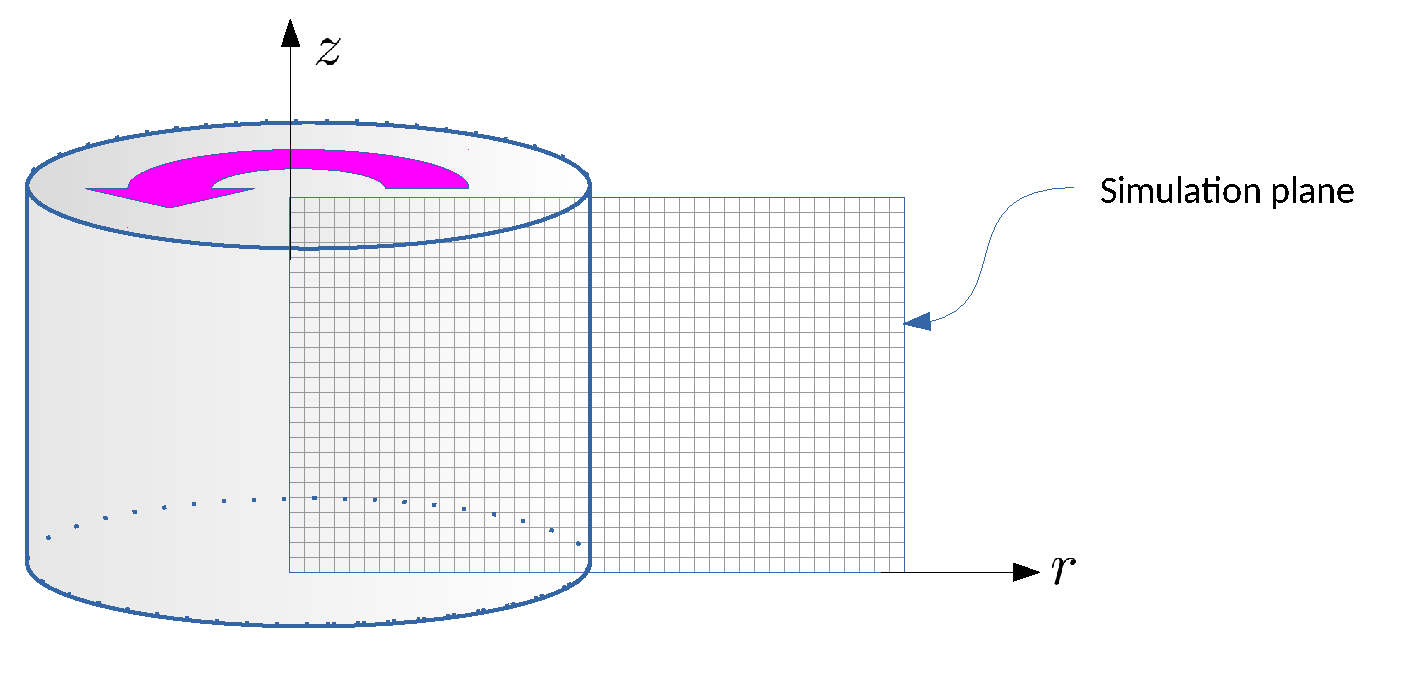
\includegraphics[width=0.8\linewidth]{axisymmetry}
\caption[The axisymmetric computational domain]
{\label{fig:axisymmetri} The axisymmetric computational domain.  Here we
  imagine that the 2-d plane rotates through the cylindrical $\theta$ angle to
  create a volume.}
\end{figure}

It is also common to do 2-d axisymmetric models---here the $r$ and $z$
coordinates from a cylindrical geometry are modeled.  Again, this
appears Cartesian, except there is a volume factor implicit in the
divergence that must be accounted for.  Our system in axisymmetric
coordinates\footnote{Some sources will call this cylindrical
  coordinates, but note that the grid is not a polar grid---it is
  still Cartesian} is:
\begin{equation}
\frac{\partial \Uc}{\partial t}
  + \frac{1}{r}\frac{\partial r \Fb^{(r)}}{\partial r}
  + \frac{\partial \Fb^{(z)}}{\partial z} = 0
\end{equation}
Expanding out the $r$ derivative, we can write this as:
\begin{equation}
\frac{\partial \Uc}{\partial t}
  + \frac{\partial \Fb^{(r)}}{\partial r}
  + \frac{\partial \Fb^{(z)}}{\partial z} = -\frac{\Fb^{(r)}}{r}
\end{equation}
Again, the primitive variable version of this expanded form is used
for the interface state prediction.  The conservative update
follows the same idea as the 1-d spherical version.  The area
and volume factors only differ from their Cartesian counterparts
in the radial direction, and take the form:
\begin{align}
A_{i-\myhalf,j} &= r_{i-\myhalf} \Delta z \\
A_{i,j-\myhalf} &= r_i \Delta z\\
V_{i,j} &= r_i \Delta r \Delta z
\end{align}
These choices of geometric factors reproduce a discretized
form of the cylindrical divergence:
\begin{equation}
\nabla \cdot {\boldsymbol{\phi}} = \frac{1}{r} \ddr{(r\phi^{(r)})} + \ddz{\phi^{(z)}}
\end{equation}
Just as with the 1-d spherical case, the pressure term in the momentum
equation needs to be treated separately from the flux, since it enters
as a gradient and not a divergence.


%-----------------------------------------------------------------------------
\section{Some Test problems}

There are a large number of standard test problems that are used to
test out our methods.  Like we say with advection, it is best to have
a problem with an analytic solution.  Here we show just a few of the most
popular test problems.

\subsection{Shock tubes}
\label{sec:euler-methods:shocktubes}

Shock tubes are Riemann problems---consider the evolution of an
initial discontinuity in the domain.  The evolution with time will
just be the solution to the Riemann problem that we described
\S~\ref{euler:sec:riemann}.  The initial conditions can be varied to
produce any combination of shocks and rarefactions as the left and
right waves.  A popular initial condition is the Sod
problem~\cite{sod:1978} which results is a right moving shock and
contact and a left moving rarefaction.

Note: it is a good test of your code's ability to preserve symmetry to
flip the initial conditions left/right and rerun.  The results should
be the same to machine precision, but atleast to roundoff error.  A
common reason for breaking symmetry is using inequalities in your code
that are biases in a direction, e.g.,
\begin{lstlisting}
if u > 0:
   # positive velocity test case
else:
   # negative or zero velocity test case
\end{lstlisting}
This has a left-right bias, since we don't handle the case where $u =
0$ separately.  A better construction would test on $u < 0$ alone, and
then have a final {\em else} clause to catch $u = 0$.

Since these tests start out with a discontinuity, they are not the
best tests to use for convergence testing.  Wherever there is an
initiali discontinuity, the limiters will kick in and drop your
method to first-order accurate.

For a general equation of state, you can still solve the Riemann
problem exactly and define analogous test problems to those commonly
used for a gamma-law gas.  Some shock tube test problems for a stellar
equation of state are shown in \cite{zingalekatz}.

For the tests shown below, we use the \hydrooned\ code described in
Appendix~\ref{app:hydro1d}.

\subsubsection{Sod problem}

The initial conditions for the Sod problem \cite{sod:1978} are:
\begin{align}
\rho_l &= 1      &  \rho_r &= 1/8 \nonumber \\
u_l   &= 0       &  u_r    &= 0   \\
p_l    &= 1      &  p_r    &= 1/10 \nonumber
\end{align}
usually with $\gamma = 1.4$\MarginPar{double check}

These result in a left wave moving contact and rightward moving
contact and shock.  The shock is not particularly strong, but this
problem is a nice demonstration of the types of hydrodynamic waves.

\begin{figure}[t]
\centering
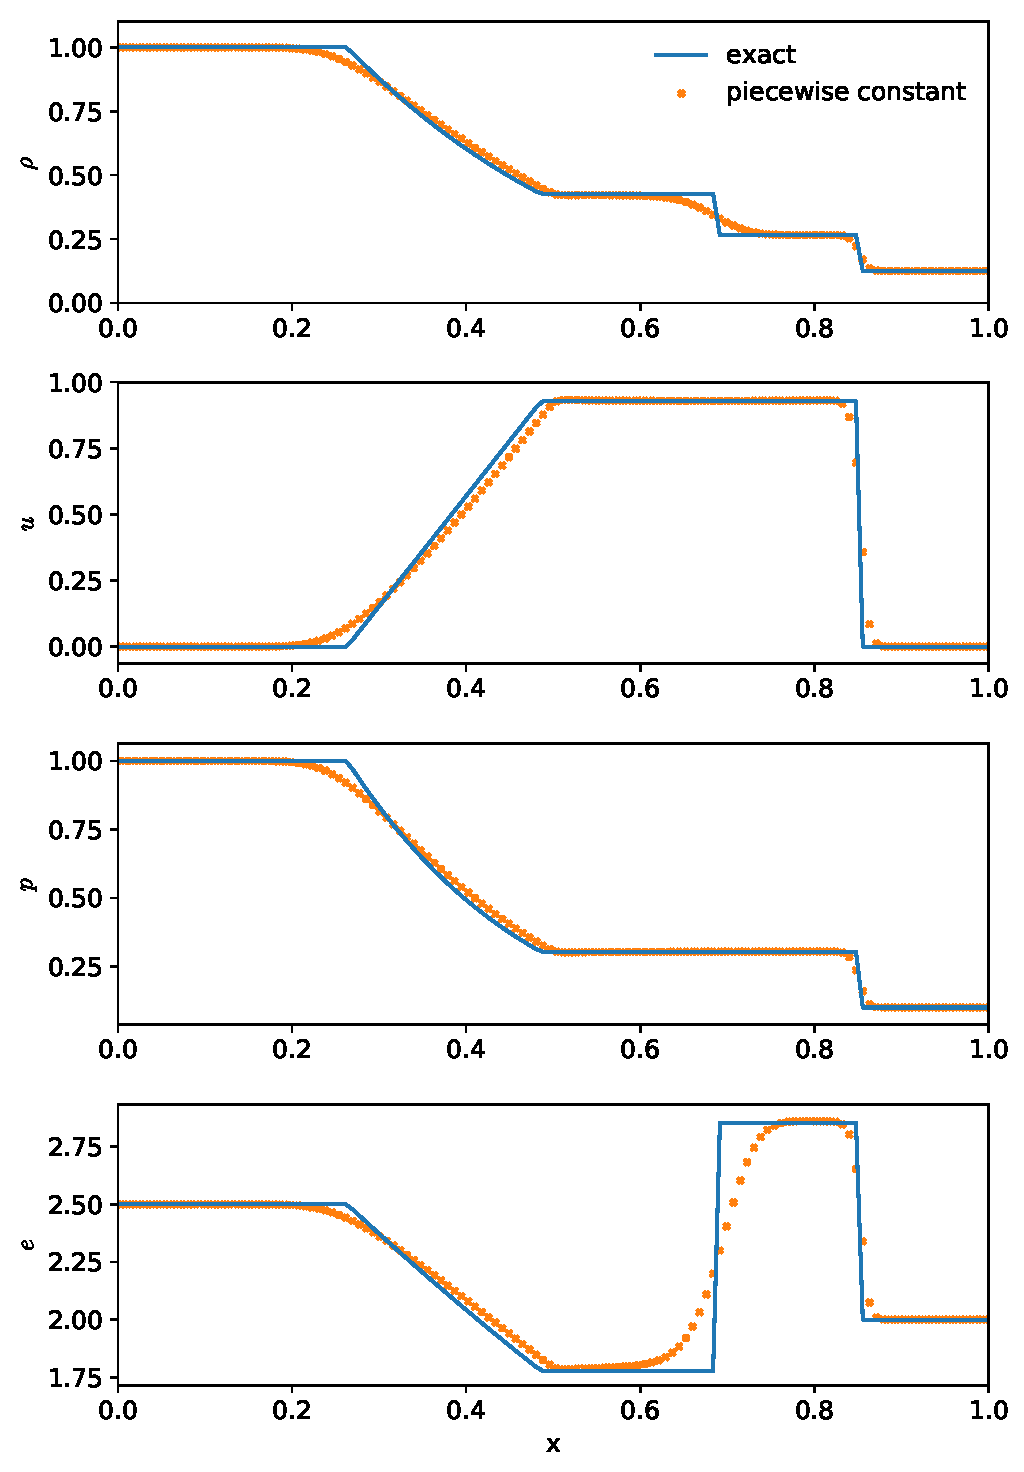
\includegraphics[width=0.7\linewidth]{hydro1d_god_sod}
\caption[Piecewise constant reconstruction Sod problem]{\label{fig:Euler:sod:god} Piecewise constant reconstruction
  with the Sod problem, using 128 zones, $\cfl = 0.8$, and the CGF
  Riemann solver.  This was run with \hydrooned\ using the {\tt sod}
  problem setup, setting {\tt godunov\_type=0} and visualized with the
  {\tt sod\_compare.py} script there.}
\end{figure}

\begin{figure}[t]
\centering
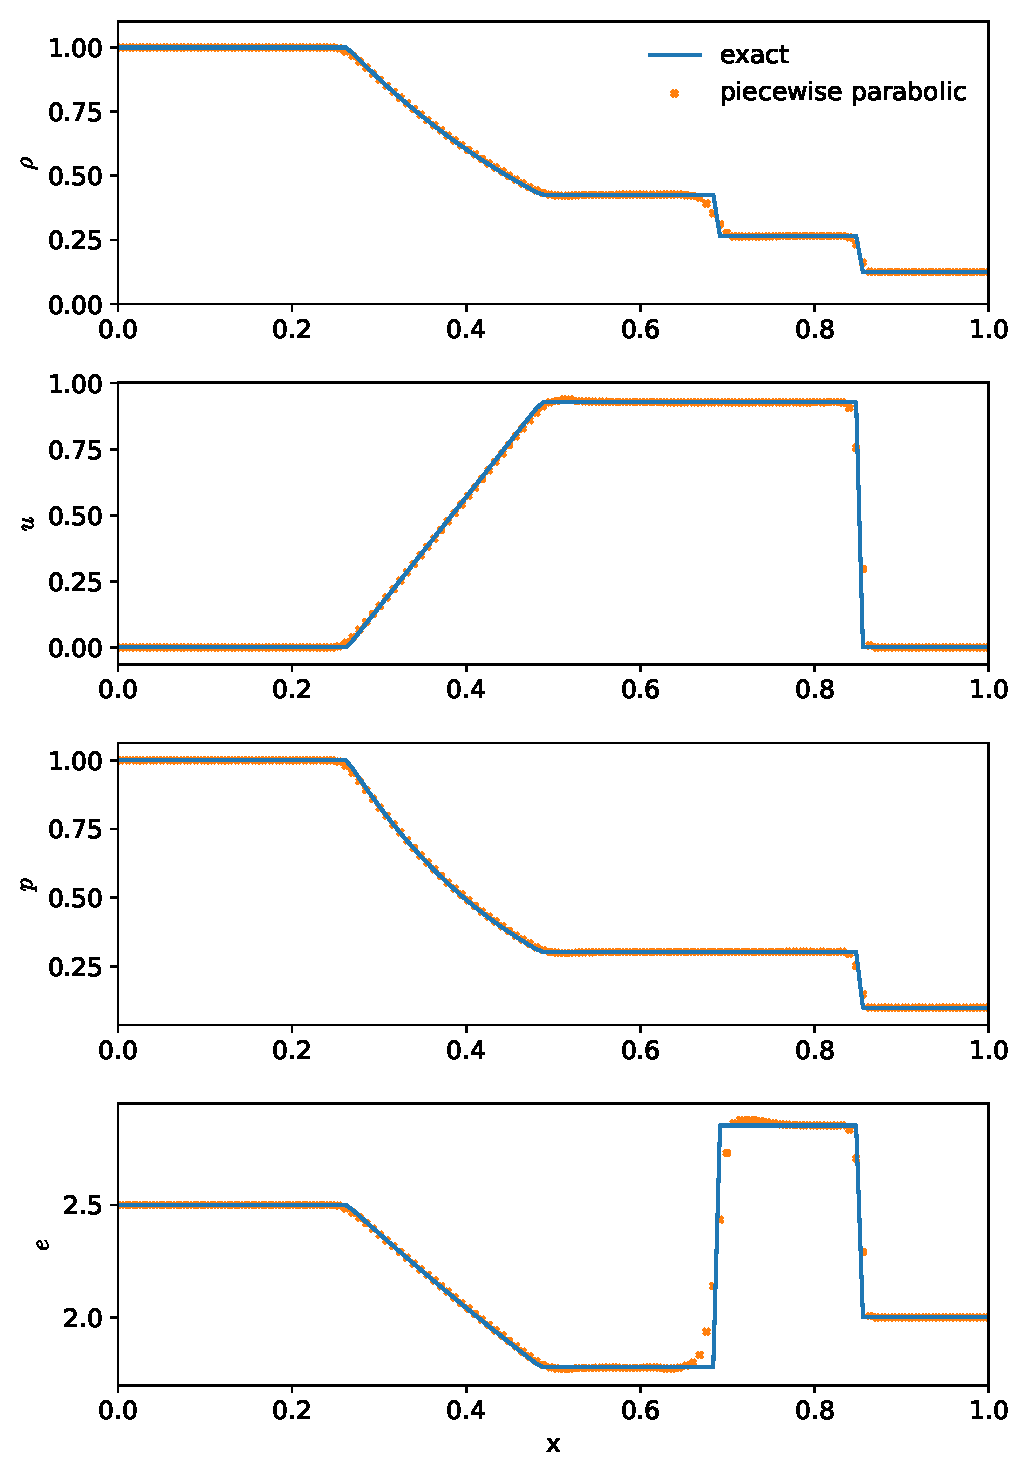
\includegraphics[width=0.7\linewidth]{hydro1d_ppm_sod}
\caption[Piecewise parabolic reconstruction Sod problem]{\label{fig:Euler:sod:ppm} Piecewise parabolic reconstruction
  with the Sod problem, using 128 zones, $\cfl = 0.8$, and the CGF
  Riemann solver.  This was run with \hydrooned\ using the {\tt sod}
  problem setup, setting {\tt godunov\_type=2} and visualized with the
  {\tt sod\_compare.py} script there.}
\end{figure}


\subsubsection{Double rarefaction}

The double rarefaction problem starts with initially diverging flow
that creates a vacuum state in the middle.  The initial conditions (as
given in \cite{toro:1997} are
\begin{align}
\rho_l &= 1      &  \rho_r &= 1 \nonumber \\
u_l    &= -2.0   &  u_r    &= 2.0   \\
p_l    &= 0.4    &  p_r    &= 0.4 \nonumber
\end{align}


\begin{figure}[t]
\centering
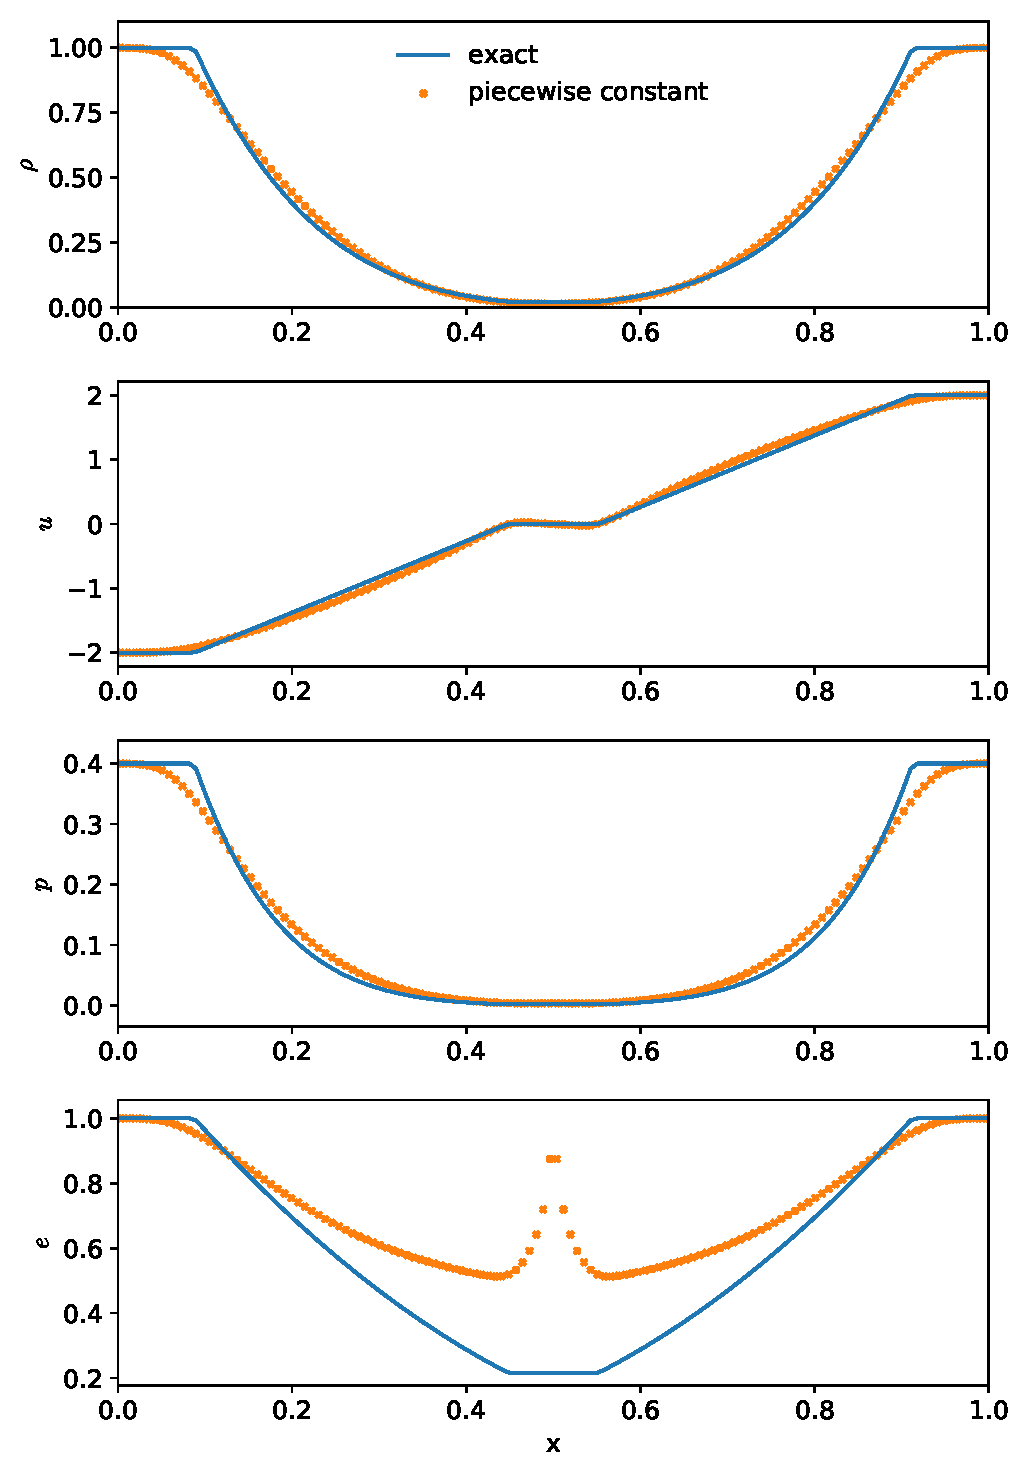
\includegraphics[width=0.7\linewidth]{hydro1d_god_double_rare}
\caption[Piecewise constant reconstruction double rarefaction problem]{\label{fig:Euler:doublerare:god} Piecewise constant
  reconstruction with the double rarefaction problem, using 128 zones,
  $\cfl = 0.8$, and the CGF Riemann solver.  This was run with
  \hydrooned\ using the {\tt sod} problem setup, setting {\tt
    godunov\_type=0} and visualized with the {\tt sod\_compare.py}
  script there.}
\end{figure}

\begin{figure}[t]
\centering
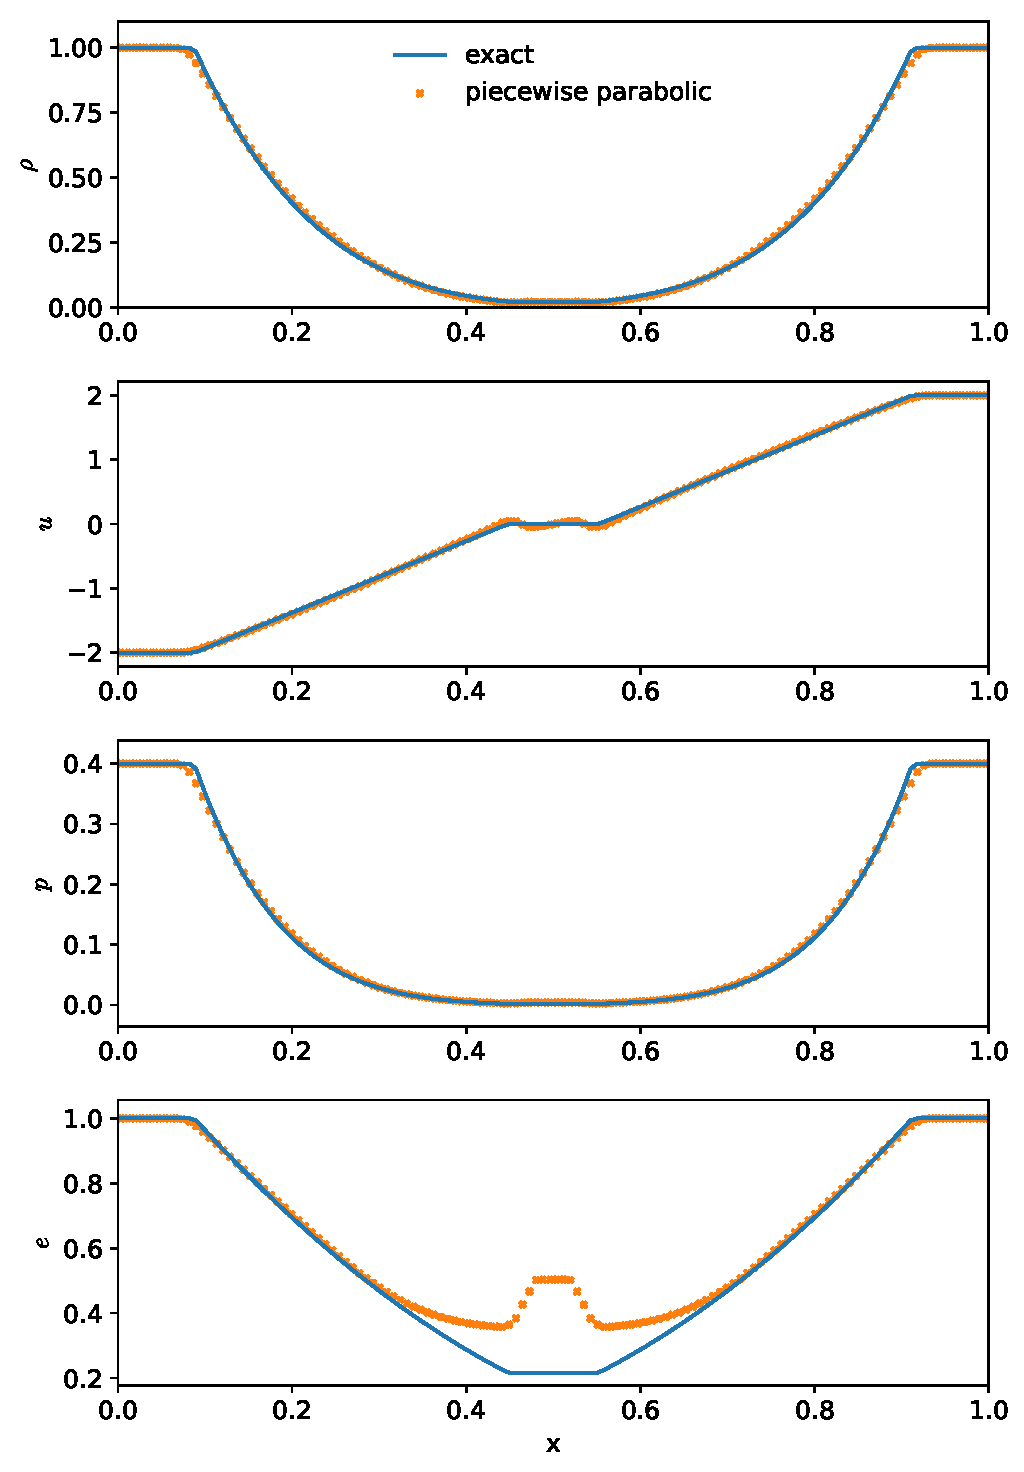
\includegraphics[width=0.7\linewidth]{hydro1d_ppm_double_rare}
\caption[Piecewise constant reconstruction double rarefaction problem]{\label{fig:Euler:doublerare:ppm} Piecewise parabolic
  reconstruction with the double rarefaction problem, using 128 zones,
  $\cfl = 0.8$, and the CGF Riemann solver.  This was run with
  \hydrooned\ using the {\tt sod} problem setup, setting {\tt
    godunov\_type=2} and visualized with the {\tt sod\_compare.py}
  script there.}
\end{figure}


\subsection{Sedov blast wave}

The Sedov (or Sedov-Taylor) blast wave~\cite{sedov:1959} is a point
explosion---energy, $\mathcal{E}_\mathrm{expl}$, is placed at a point
in a uniform domain.  A spherical shockwave propagates outward,
evacuating the region in the center.  The Sedov problem also has an
analytic solution\footnote{See \cite{timmes_sedov_code} for a nice
  code to general the solutions}, and this problem is a good way of
testing out the geometric factors for 1-d spherical and 2-d
axisymmetric geometries.

\begin{figure}[t]
\centering
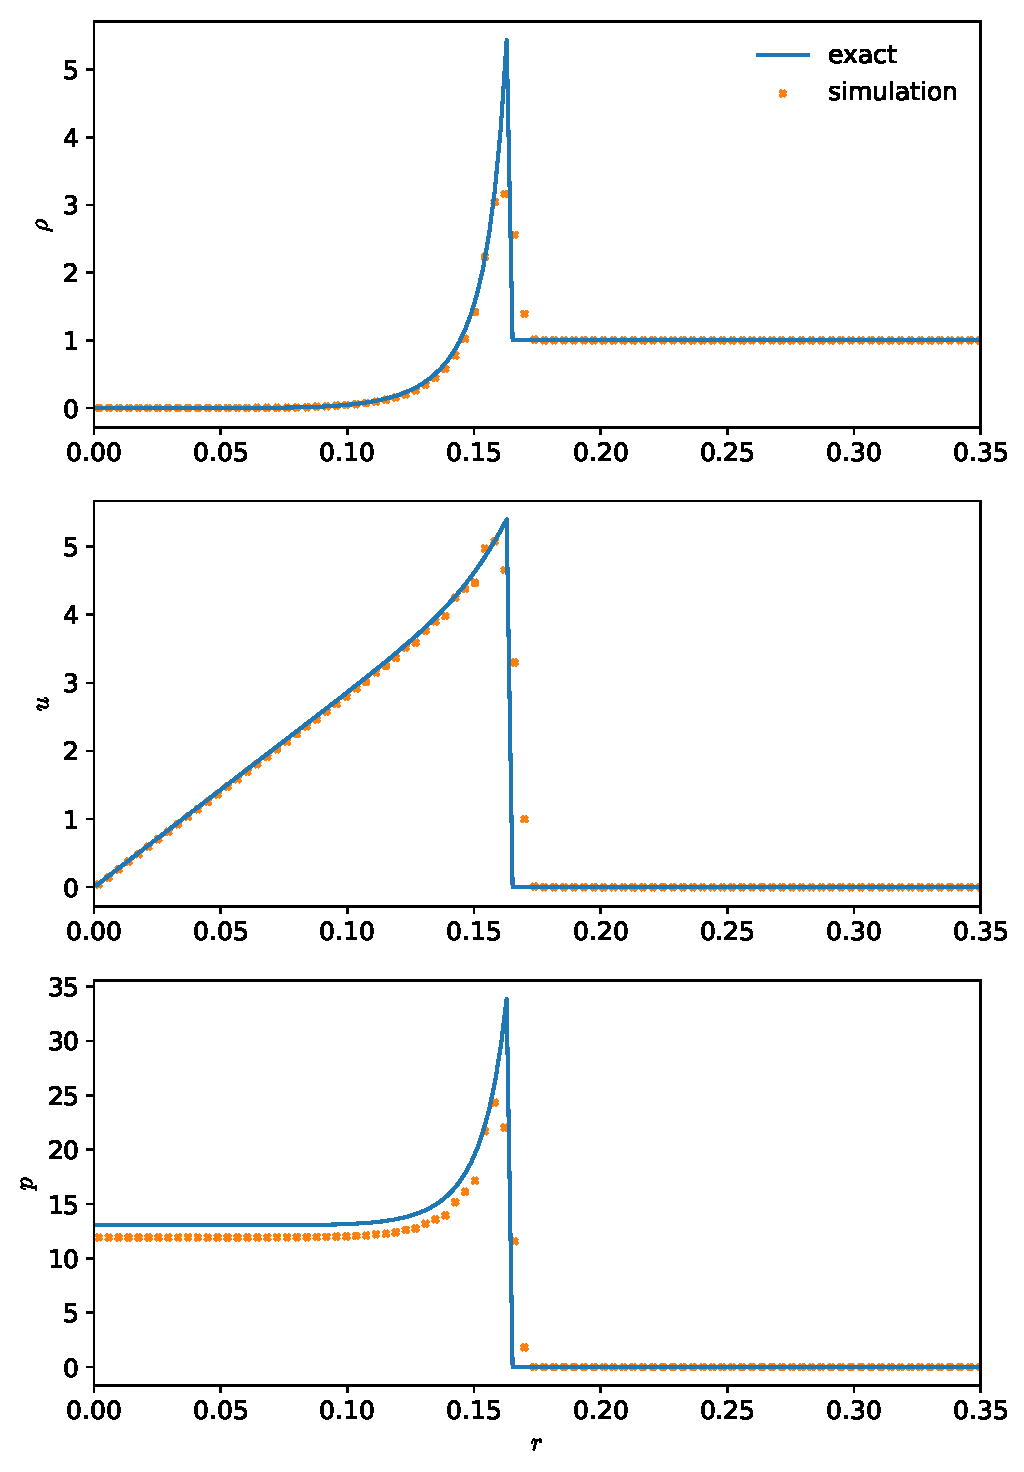
\includegraphics[width=0.7\linewidth]{hydro1d_sedov_1dsph}
\caption[1-d spherical Sedov problem]{\label{fig:Euler:sedov1d} 1-d Sedov explosion with
  piecewise parabolic reconstruction, using 128 zones (on $r \in
  [0,1]$), $\cfl = 0.8$, and the CGF Riemann solver.  This was run
  with \hydrooned\ using the {\tt sedov} problem setup and visualized
  with the {\tt sedov\_compare.py} script there.  The 1-d spherical
  geometry used makes this act as if it were a sphere.}
\end{figure}

The major difficulty with initializing the Sedov problem is
representing a point, where all the energy desposited, on the grid.
If you just initialize a singe zone, then the size of the point
changes as you change resolution.  Additionally, in 2- or 3-d
Cartesian coordinates, the point will be squared off.  A standard way
of initializing this (see, e.g., \cite{omang:2006}) is to imagine the
energy deposition inflating a region of radius $r_\mathrm{init}$ like
a balloon, resulting in an energy density, $E =
\mathcal{E}_\mathrm{expl}/V_\mathrm{init}$, where $V_\mathrm{init} =
4\pi r_\mathrm{init}^3/3$ for a spherical blast wave and
$V_\mathrm{init} = \pi r_\mathrm{init}^2$ for a cylindrical blast
wave. Then the pressure is
\begin{equation}
p = \frac{\mathcal{E}_\mathrm{expl}}{V_\mathrm{init}} (\gamma - 1)
\end{equation}


Figure~\ref{fig:Euler:sedov1d} shows the solution to the Sedov problem
in 1-d in a spherical geometry.  This is compared to the spherical
Sedov solution (solid line). There is good agreement in the position of the
shock and density and velocity profiles.  The pressure behind the shock
is a little low---this is likely an artifact of the initialization process.

In 2-d, we run the problem in Cartesian coordinates---this produces a cylindrical
blast wave.  Figure~\ref{fig:Euler:sedov2d} shows the solution in 2-d.
\begin{figure}[t]
\centering
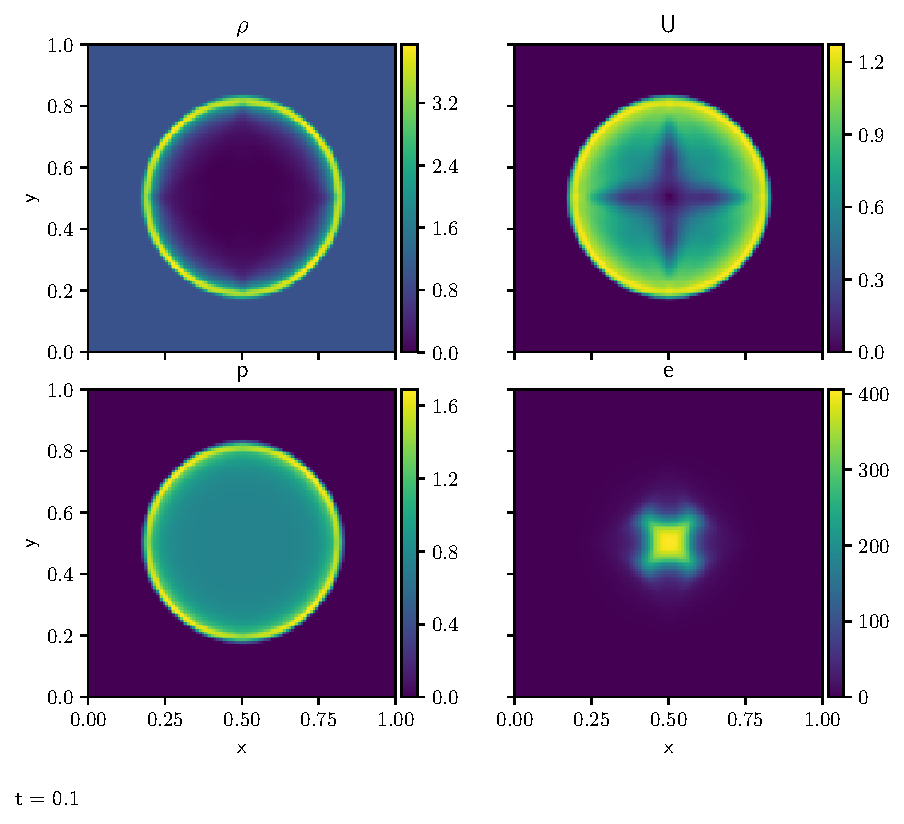
\includegraphics[width=0.85\linewidth]{sedov_pyro}
\caption[2-d cylindrical Sedov problem]{\label{fig:Euler:sedov2d} 2-d Sedov explosion with
  piecewise linear reconstruction, using 128$^2$ zones (on $r \in
  [0,1]\times[0,1]$), $\cfl = 0.8$, and the HLLC Riemann solver.  This was run
  with \pyro\ as {\tt ./pyro.py compressible sedov inputs.sedov}.  An initial
  perturbation size of $r_\mathrm{init} = 0.01$ was used.}
\end{figure}
The density and pressure look very symmetric.  In the velocity magnitude
plot, we see an imprint of the grid along coordinate axes, and likewise
in the internal energy.  The bump in internal energy near the origin arises
because of the error in defining $e$ from $E$ and $U$.  We can produce an angle-averaged
profile of this and compare to the analytic solution, shown in Figure~\ref{fig:Euler:sedov2d_compare}.

\begin{figure}[t]
\centering
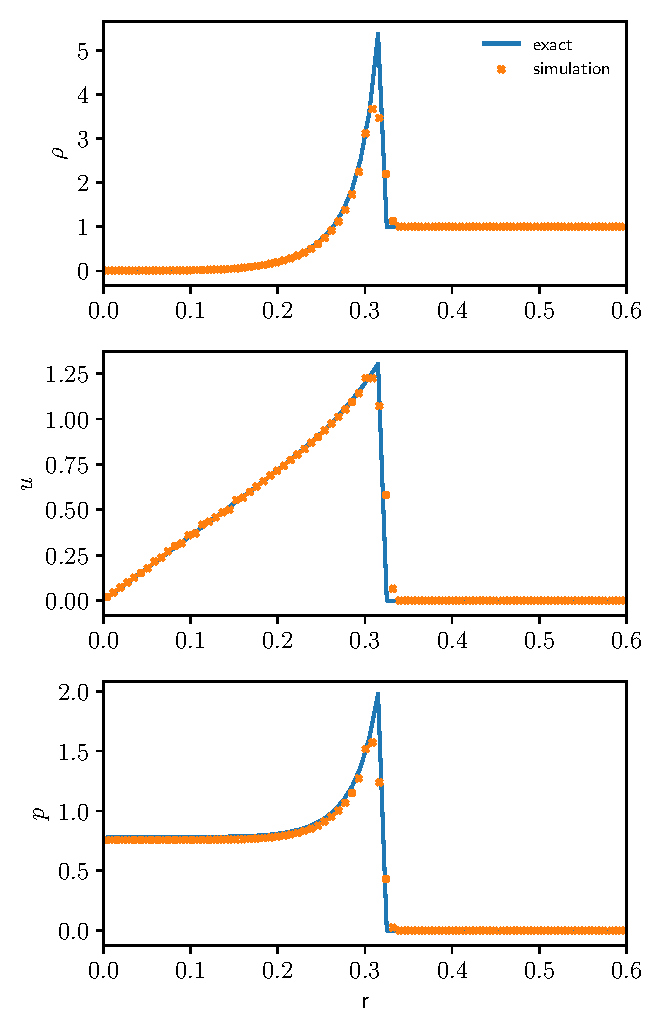
\includegraphics[width=0.75\linewidth]{sedov_compare}
\caption[2-d cylindrical Sedov problem]{\label{fig:Euler:sedov2d_compare} Angle-average 
  profile for the 2-d Sedov explosion from Figure~\ref{fig:Euler:sedov2d} shown
  with the analytic solution.  This was constructed using the {\tt sedov\_compare.py}
  script in \pyro.}
\end{figure}


\subsection{Advection}

We can run a simple advection test analogous to the tests we used in
Ch.~\ref{ch:advection}.  However, because we are now doing hydrodynamics,
we need to suppress the dynamics.  This is accomplished by putting the 
profile we want to advect in the density field and then put it in
pressure equilibrium by adjusting the internal energy.  For example, consider
a Gaussian profile.  We initialize the density as:
\begin{equation}
\rho = (\rho_1 - \rho_0) e^{-(x - x_c)^2/\sigma^2} + \rho_0
\end{equation}
To advect the profile to the right, we choose a constant velocity,
\begin{equation}
u = u_0
\end{equation}
and to suppress dynamics, we make the pressure constant,
\begin{equation}
p = p_0
\end{equation}
Finally, we compute the total energy as
\begin{equation}
\rho E = \frac{p}{\gamma - 1} + \frac{1}{2}\rho u^2
\end{equation}

\begin{figure}[t]
\centering
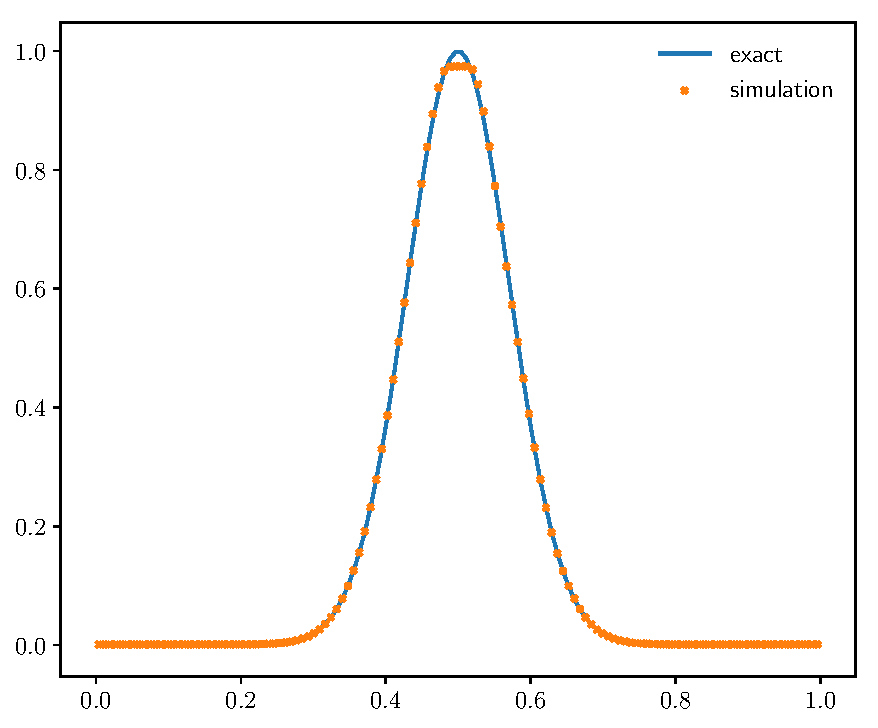
\includegraphics[width=0.7\linewidth]{advect_hydro1d}
\caption[Simple advection test]{\label{fig:Euler:advect:1d} Piecewise
  parabolic reconstruction with an advection test, using 128 zones,
  $\cfl = 0.8$, and the CGF Riemann solver.  A Gaussian profile was
  advected for 10 periods.  This was run with \hydrooned\ using the
  {\tt advect} problem setup and
  visualized with the {\tt advect\_compare.py} script there.}
\end{figure}

Figure~\ref{fig:Euler:advect:1d} shows an example of a Gaussian
profile advected for 10 periods.  The initial conditions used $\rho_0
= 10^{-3}$, $\rho_1 = 1$, $p_0 = 10^{-6}$, $u_0 = 1$, and $\sigma =
0.1$ (these coincide with the choices used in \cite{flash}).  The
non-zero value for the ambient density, $\rho_0$, ensures that any
quantities that are derived by dividing by density remain
well-defined.  The result is similar to what we saw when we considered
pure advection---the shape is mostly preserved, but the peak of the
Gaussian is clipped.

\subsection{Slow moving shock}

Slow moving (or stationary) shocks can be difficult to model, as
oscillations can be setup behind the shock (this is discussed a little
in \cite{colellawoodward:1984,leveque:2002}).  We can produce a slow
moving shock as a shock tube, and we can use the jump conditions 
across a shock that were derived for the Riemann problem to find the
conditions to setup a stationary (or slow-moving) shock.  

The speed of a right-moving shock was found (see
Eq.~\ref{eq:euler:shockspeedjump}) as:
\begin{equation}
S = u_r + c_r \left [ \left ( \frac{p_\star}{p_r} \right ) \frac{\gamma+1}{2\gamma} + \frac{\gamma-1}{2\gamma} \right ]^{\myhalf}
\end{equation}
We want $S = 0$, which allows us to express the pre-shock velocity, $u_r$, as:
\begin{equation}
u_r = -c_r \left [ \left ( \frac{p_\star}{p_r} \right ) \frac{\gamma+1}{2\gamma} + \frac{\gamma-1}{2\gamma} \right ]^{\myhalf}
\end{equation}
We have the freedom to choose the density and pressure ahead of the
shock, $\rho_r$ and $p_r$, which in turn gives us $c_r$.  Next, we can
pick the strength of the shock by choosing the jump in pressure,
$p_\star/p_r$.  Together, this allows us to compute $u_r$, and thus we
know the entire pre-shock state.  We can compute the post-shock state
(which was the star state when we discussed the Riemann problem) using
the jump conditions, Eqs.~\ref{eq:euler:shockrhojump} and
\ref{eq:euler:shockujump}.\footnote{The script
  \href{https://github.com/zingale/hydro_examples/blob/master/compressible/slow_shock.py}{\tt
    slow\_shock.py} will find the initial conditions to generate a
  stationary shock.}

For a pressure jump of 100 across a shock, the following conditions will
generate a stationary right-facing shock (with $\gamma = 1.4$):
\begin{align}
\rho_l &= 5.6698      &  \rho_r &= 1 \nonumber \\
u_l   &= -1.9336      &  u_r    &= -10.9636   \\
p_l    &= 100         &  p_r    &= 1 \nonumber
\end{align}

By adjusting the velocity of both the left and right state, we can
produce a strong shock that moves slowly across the grid.  For
instance, a shock with $S = 0.4$ results from
\begin{align}
\rho_l &= 5.6698      &  \rho_r &= 1 \nonumber \\
u_l   &= -1.5336      &  u_r    &= -10.5636   \\
p_l    &= 100         &  p_r    &= 1 \nonumber
\end{align}

\begin{figure}[t]
\centering
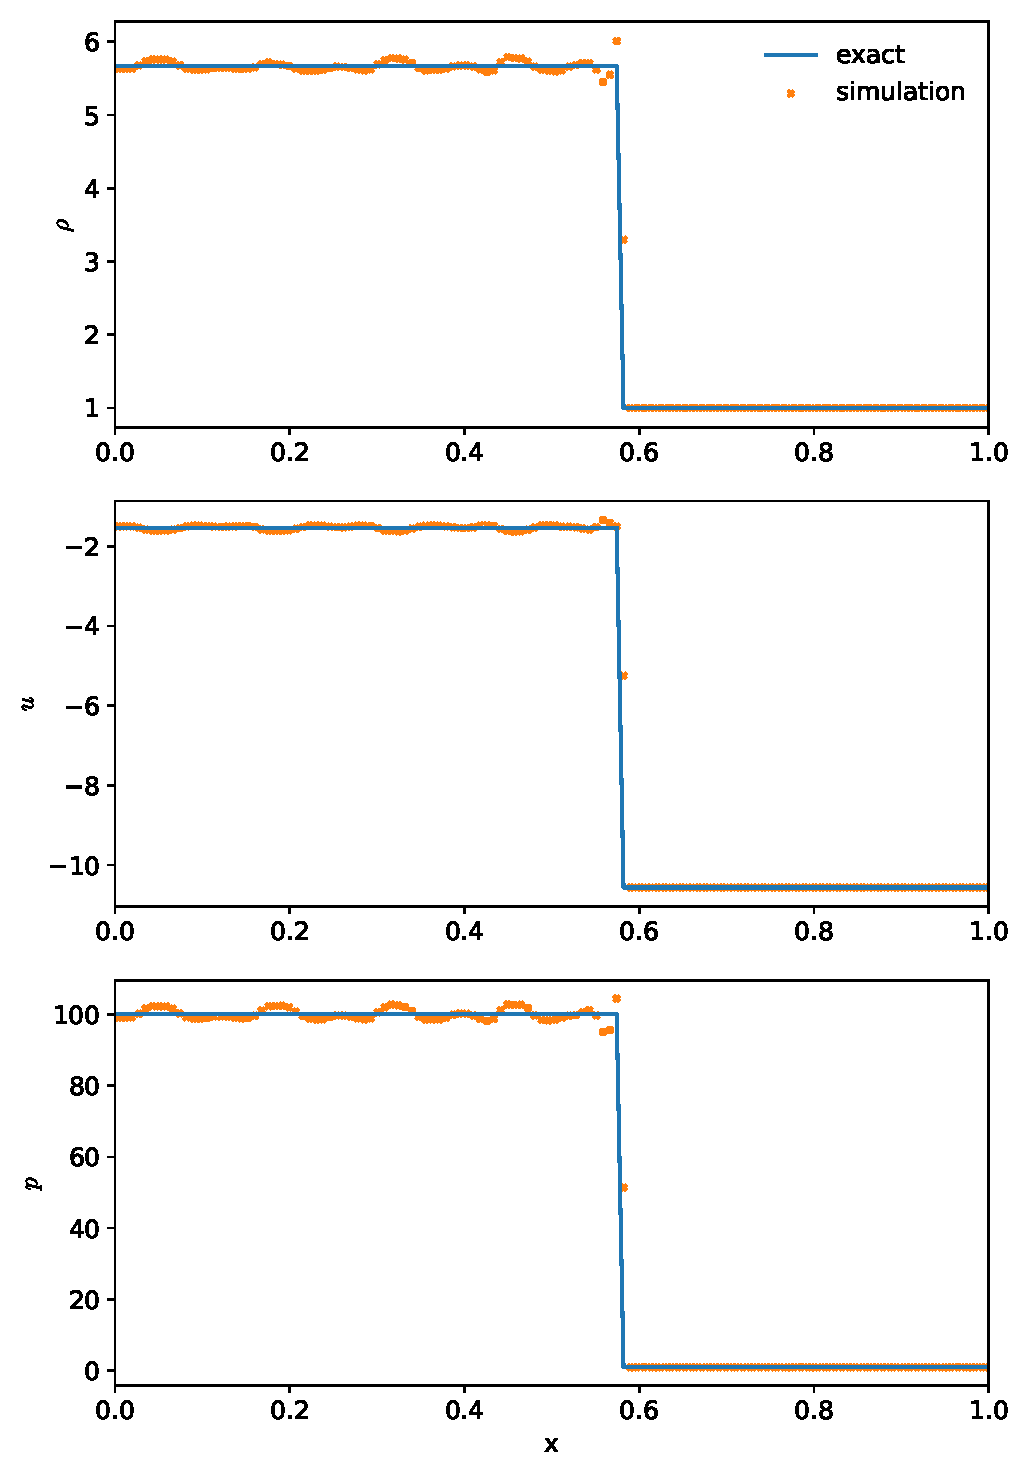
\includegraphics[width=0.7\linewidth]{slowshock}
\caption[1-d spherical Sedov problem]{\label{fig:Euler:slowshock:ppm} 1-d slow moving shock
  problem with
  piecewise parabolic reconstruction, using 128 zones (on $r \in
  [0,1]$), $\cfl = 0.8$, and the CGF Riemann solver.  This was run
  with \hydrooned\ using the {\tt sod} problem setup and visualized
  with the {\tt sod\_compare.py} script there.}
\end{figure}


\subsection{Two-dimensional Riemann problems}

Several different 2-d Riemann problems were introduced in
\cite{hydro_test_quad}, to explore the multi-dimensional
interactive of the different hydrodynamic waves.  These
problems initialize the 4 quadrants of the domain with different
states, and watch the ensuing evolution.  There are some
analytic estimates that can be compared to, but also these
tests can provide a means of assessing the symmetry of 
a code in the presence of complex flows.  We use the setup
corresponding to {\em configuration 3} in that paper (this
same setup is used in \cite{leveque:1997}).

\begin{figure}[t]
\centering
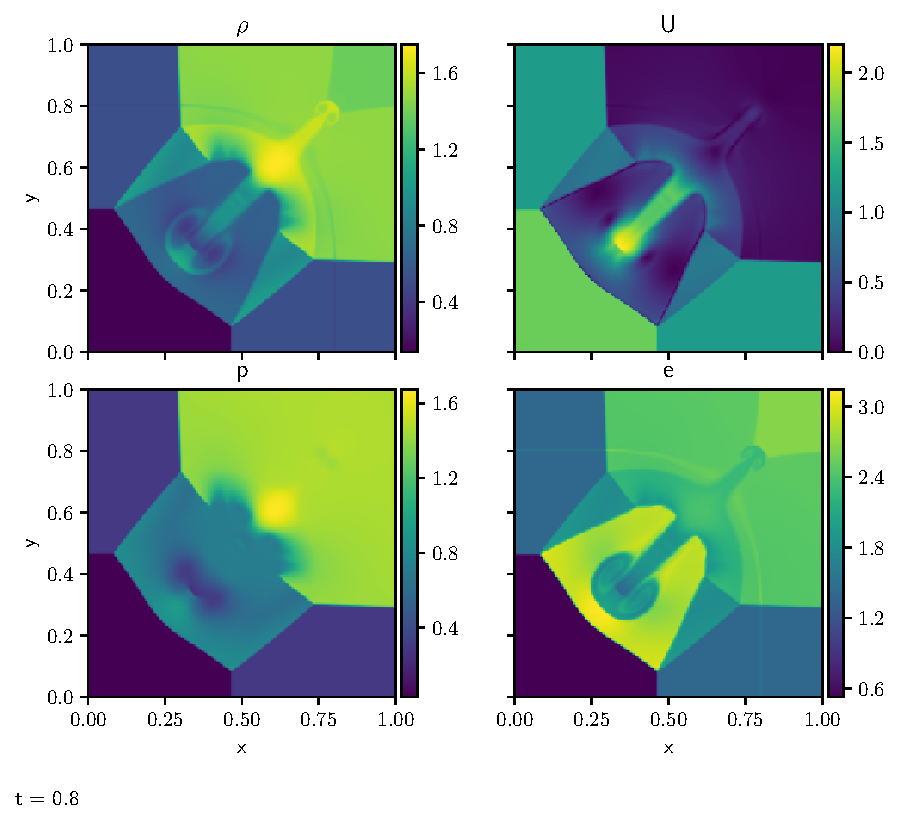
\includegraphics[width=0.85\linewidth]{quad}
\caption{\label{fig:Euler:quad} Two-dimensional Riemann problem
from \cite{hydro_test_quad}.}
\end{figure}

\ifdefined \debugmode
\subsection{Odd-even decoupling}

\subsection{Gresho vortex}

The Gresho vortex is a vortex in with a stabilizing pressure gradient
designed such that the overall structure is unchanging in time.  It
has a nice feature in that it allows you to set the Mach number of
the flow as one of the parameters.


\subsection{Hydrostatic equilibrium}

Hydrodynamics codes can have a difficult time keeping an atmosphere in
hydrostatic equilibrium.  This is because any departure from $\nabla p
= \rho {\bf g}$ due to truncation error in the method will be seen as an
acceleration by the momentum equation:
\begin{equation}
\rho \DDt{\Ub} = \rho {\bf g} - \nabla p
\end{equation}
The result will be growing velocities in the atmosphere, which can
overwhelm any signal in the flow that you are interested in studying.
Since this acceleration is driven by truncation error, higher
resolution will result in lower velocities.

% top of the star

% scale height resolved -- do uniform T atmosphere


%\subsection{Rayleigh-Taylor instability}

\fi


%-----------------------------------------------------------------------------
\section{Method of lines integration and higher order}
\label{sec:comp:mol}
Just like we explored with linear advection (\S~\ref{adv:sec:mol_2d}),
instead of doing the characteristic tracing, we could rely on the
integrator to do the work for us.


Discretizing our system in space leads to the following system:
\begin{equation}
\frac{d\Uc_{i,j}}{dt} = -\frac{\Fb^{(x)}(\Uc_{i+\myhalf,j}) - \Fb^{(x)}(\Uc_{i-\myhalf,j})}{\Delta x}
                      -\frac{\Fb^{(y)}(\Uc_{i,j+\myhalf}) - \Fb^{(y)}(\Uc_{i,j-\myhalf})}{\Delta y}
\end{equation}
Note that there is no time superscript in the $\Uc$ used to evaluate the
fluxes on the righthand side---we have not done any time
discretization yet.  Now we can use an ODE integrator to solve this system.

Consider
second-order Runge-Kutta.  We evaluate two slopes,
\begin{alignat}{3}
{\bf k}_1 &= \Delta t \bigg [ &-&\frac{\Fb^{(x)}(\Uc^n_{i+\myhalf,j})
                               - \Fb^{(x)}(\Uc^n_{i-\myhalf,j})}{\Delta x} \nonumber \\
    &\,                 &-&\frac{\Fb^{(y)}(\Uc^n_{i,j+\myhalf})
                               - \Fb^{(y)}(\Uc^n_{i,j-\myhalf})}{\Delta y} \bigg ] \\
{\bf k}_2 &= \Delta t \bigg [ &-&\frac{\Fb^{(x)}([\Uc^n + {\bf k}_\myhalf]_{i+\myhalf,j})
                               - \Fb^{(x)}([\Uc^n + {\bf k}_\myhalf]_{i-\myhalf,j})}{\Delta x} \nonumber \\
    &\,                 &-&\frac{\Fb^{(y)}([\Uc^n + {\bf k}_\myhalf]_{i,j+\myhalf})
                               - \Fb^{(y)}([\Uc^n + {\bf k}_\myhalf]_{i,j-\myhalf})}{\Delta y} \bigg ]
\end{alignat}
and then
\begin{equation}
\Uc^{n+1}_{i,j} = \Uc^n_{i,j} + {\bf k}_2
\end{equation}
In the construction of the interface states, $\Uc^n_{i+\myhalf,j}$ or $[\Uc^n
+ {\bf k}_\myhalf]_{i+\myhalf,j}$, there is no explicit transverse term, since that
arose from Taylor expanding $\Uc^n_{i,j}$ in time through $\Delta t/2$.
Instead, we simply construct these interface states using a
one-dimensional reconstruction and solve a Riemann problem at each
interface.  The evaluation of the second slope, ${\bf k}_2$, implicitly
includes the transverse information since we add ${\bf k}_\myhalf$ to
$\Uc^n_{i,j}$ before doing the prediction to the interfaces.  Also note,
however, that in this construction of the interface states, there is
no characteristic projection, since that arises from predicting the
interface states forward in time.  Again, these interface states are
at a constant time, not predicted into the future.

Generally speaking we want the order of accuracy in time to match that
in space.  The fourth-order Runge-Kutta method is a popular method for
integrating ODEs, so it makes sense to couple this with a
fourth-order-in-space method.  However, going higher-order than
second-order is more challenging.  The key issue is that we can no
longer simply approximate the cell average as the cell-center value,
i.e., $\langle \phi\rangle_i \ne \phi_i$.  This comes into play, for
instance, in translating between the conserved and primitive variables.
A fully fourth-order method is presented in ~\cite{mccorquodalecolella}

Note that when using a Runge-Kutta method-of-lines integrator for the
time-discretization of a multidimensional system, the timestep is
actually more restrictive than the cases presented above that
predicted the interface states to the half-time and performed
characteristic tracing.  Titarev \& Toro \cite{titarevtoro} claim that
you need $0 < C < \myhalf$ for 2-d flows and $0 < C < 1/3$ for 3-d flows.

An additional complexity arises when doing multiphysics.  Often we
split the different physical processes up and treat them in turn.
There are standard methods to do this with second-order accuracy in time,
but higher-order is more tricky.





\section{Thermodynamic issues}

\subsection{Defining temperature}

  Although not needed for the pure
  Euler equations, it is sometimes desirable to define the temperature
  for source terms (like reactions) or complex equations of state.
  The temperature can typically be found from the equation of state
  given the internal energy:
  \begin{eqnarray}
  e &=& E - \frac{1}{2} u^2 \\
  T &=& T(e, \rho)
  \end{eqnarray}
  Trouble can arise when you are in a region of flow where the kinetic
  energy dominates (high Mach number flow).  In this case, the $e$ defined
  via subtraction can become negative due to truncation error in the
  evolution of $u$ compared to $E$.  In this instance, one must either
  impose a floor value for $e$ or find an alternate method of deriving
  it.

  In~\cite{bryan:1995}, an alternate formulation of the Euler equations
  is proposed.  Both the total energy equation {\em and} the internal
  energy equation are evolved in each zone.  When the flow is dominated
  by kinetic energy, then the internal energy from the internal energy
  evolution equation is used.  The cost of this is conservation---the
  internal energy is not a conserved quantity, and switching to it
  introduces conservation of energy errors.

\subsection{General equation of state}

The above methods were formulated with a constant gamma equation of
state.  A general equation of state (such as degenerate electrons)
requires a more complex method.  Most methods are designed to 
reduce the need to call a complex equation of state frequently,
and work by augmenting the vector of primitive variables with 
additional thermodynamic information.  There are two parts of the 
adaption to a general equation of state: the interface states and 
the Riemann problem. 

\subsubsection{Carrying $\gamma_e$}


The classic prescription for
extending this methodology is presented by Colella and
Glaz~\cite{colellaglaz:1985}.  They construct a thermodynamic index,
\begin{equation}
\gamma_e = \frac{p}{\rho e} + 1
\end{equation}
and derive an evolution equation for $\gamma_e$ (C\&G, Eq.\ 26).
We can derive a similar expression as
\begin{align}
\frac{D\gamma_e}{Dt} &= \frac{D}{Dt} \left ( \frac{p}{\rho e} + 1 \right )
   = - \frac{p}{(\rho e)^2} \frac{D(\rho e)}{Dt} + \frac{1}{\rho e} \frac{Dp}{Dt} \nonumber \\
   &= (\gamma_e - 1) (\gamma_e  - \Gamma_1) \nabla \cdot \Ub \label{eq:gammae}
\end{align}
where we used Eqs.~\ref{eq:euler:pgeneral} and \ref{eq:euler:econs}, and the definition
of the sound speed.

This evolution equation is used to predict $\gamma_e$ to interfaces,
and these interface values of $\gamma_e$ are used in the Riemann
solver presented there to find the fluxes through the interface.  A
different adiabatic index (they call $\Gamma$, we call $\Gamma_1$)
appears in the definition of the sound speed.  They argue that this
can be brought to interfaces in a piecewise constant fashion while
still making the overall method second order, since $\Gamma_1$ does
not explicitly appear in the fluxes (see the discussion at the top of
page 277).

We can derive the characteristic structure of this system for use
in the tracing in the construction of interface states%
\footnote{A {\sf Jupyter} notebook using {\sf SymPy} that derives these
eigenvectors is available here:
\hydroexdoit{\href{https://github.com/zingale/hydro_examples/blob/master/compressible/euler-generaleos.ipynb}{euler-generaleos.ipynb}}}.
If we write 
our system as
\begin{equation}
\qb = \left ( \begin{array}{c} \tau \\ u \\ p \\ \gamma_e \end{array} \right )
\end{equation}
(we use $\tau = 1/\rho$ here for consistency with CG), we have
\begin{equation}
\Ab = \left ( \begin{array}{cccc} u & -\tau    & 0      & 0 \\
                                0 & u        & \tau   & 0 \\
                                0 & c^2/\tau & u      & 0 \\
                                0 & -\alpha  & 0      & u
            \end{array} \right )
\end{equation}
where we define $\alpha = (\gamma_e - 1)(\gamma_e - \Gamma_1)$ for
convenience.  The right eigenvectors are:
\begin{equation}
\rb^\evm = \left( \begin{array}{c} 1\\ {c}/{\tau}\\ -{c^{2}}/{\tau^{2}}\\ {\alpha}/{\tau}\end{array}\right)
%
\qquad
\rb^\evz = \left( \begin{array}{c} 1\\0\\0\\0 \end{array}\right)
%
\qquad
\rb^\evzs{\gamma_e} = \left( \begin{array}{c} 0\\0\\0\\1\end{array}\right)
%
\qquad
\rb^\evp = \left( \begin{array}{c} 1\\ -{c}/{\tau}\\ -{c^{2}}/{\tau^{2}}\\ {\alpha}/{\tau} \end{array}\right )
\end{equation}
and corresponding left eigenvectors are:
\begin{align}
\lb^\evm &= \left( \begin{array}{cccc} 0 & \frac{\tau}{2 c} & - \frac{\tau^{2}}{2 c^{2}} & 0\end{array}\right) \\
%
\lb^\evz &= \left( \begin{array}{cccc} 0 & \frac{\tau}{2 c} & - \frac{\tau^{2}}{2 c^{2}} & 0\end{array}\right) \\
%
\lb^\evzs{\gamma_e} &= \left( \begin{array}{cccc} 0 & 0 & \frac{\alpha \tau}{c^{2}} & 1\end{array}\right) \\
%
\lb^\evp &= \left ( \begin{array}{cccc} 0 & - \frac{\tau}{2 c} & - \frac{\tau^{2}}{2 c^{2}} & 0\end{array}\right)
\end{align}

\subsubsection{Carrying $(\rho e)$}

Alternately, the Castro paper~\cite{almgren:2010} relies on an idea
from an unpublished manuscript by Colella, Glaz, and Ferguson that
predicts $\rho e$ to edges in addition to $\rho$, $u$, and $p$.  Since
$\rho e$ comes from a conservation-like equation
(Eq.~\ref{eq:euler:econs}), predicting it to the interface in the
unsplit formulation is straightforward.  This over-specifies the
thermodynamics, but eliminates the need for $\gamma_e$.


With the addition of $\rho e$, our system becomes:
\begin{equation}
\qb = \left ( \begin{array}{c} \rho \\ u \\ p \\ \rho e \end{array} \right )
%
\qquad
%
\Ab = \left ( \begin{array}{cccc} u & \rho     & 0      & 0 \\
                                0 & u        & 1/\rho & 0 \\
                                0 & \rho c^2 & u      & 0 \\
                                0 & \rho h   & 0      & u
            \end{array} \right )
\end{equation}
where $h = e + p/\rho$ is the specific enthalpy.  The eigenvalues of this
system are:
\begin{equation}
\lambda^\evm = u - c \qquad
\lambda^\evz = u  \qquad
\lambda^\evzs{\rho e} = u  \qquad
\lambda^\evp = u + c
\end{equation}
and the eigenvectors are:
\begin{equation}
\rb^\evm = \left ( \begin{array}{c} 1 \\ -c/\rho \\ c^2 \\ h \end{array} \right )
\qquad
\rb^\evz = \left ( \begin{array}{c} 1 \\ 0 \\ 0 \\ 0 \end{array} \right )
\qquad
\rb^\evzs{\rho e} = \left ( \begin{array}{c} 0 \\ 0 \\ 0 \\ 1 \end{array} \right )
\qquad
\rb^\evp = \left ( \begin{array}{c} 1 \\ c/\rho \\ c^2 \\ h \end{array} \right )
\end{equation}
and
\begin{eqnarray}
&&
\lb^\evm = ( \begin{array}{cccc} 0 & -\frac{\rho}{2c} & \frac{1}{2c^2} & 0
            \end{array} ) \nonumber \\
&&
\lb^\evz = ( \begin{array}{cccc} 1 & 0 & -\frac{1}{c^2} & 0
            \end{array} ) \nonumber \\
&&
\lb^\evzs{\rho e} = ( \begin{array}{cccc} 0 & 0 & -\frac{h}{c^2} & 1
            \end{array} ) \nonumber \\
&&
\lb^\evp = ( \begin{array}{cccc} 0 & \frac{\rho}{2c} & \frac{1}{2c^2} & 0
            \end{array} )
\end{eqnarray}
Remember that the state variables in the $\qb$ vector are mixed into the
other states by $\lb \cdot \qb$.  Since all $\lb^{(\nu)}$'s have $0$ in the
$\rho e$ `slot' (the last position) except for $\lb^\evzs{\rho e}$, and the
corresponding $\rb^\evzs{\rho e}$ is only non-zero in the $\rho e$ slot, this
means that $\rho e$ is not mixed into the other state variables.  This
is as expected, since $\rho e$ is not needed in the system.

Also recall that the jump carried by the wave $\nu$ is proportional
to $\rb^{(\nu)}$---since $\rb^\evm$, $\rb^\evzs{\rho e}$, and $\rb^\evp$ have
non-zero $\rho e$ elements, this means that $\rho e$ jumps across
these three waves.

Working through the sum for the $(\rho e)$ state, and using a $\sim$ to
denote the reference states, we arrive at:
\begin{align}
(\rho e)_{i+\myhalf,L}^{n+\myhalf} = \widetilde{(\rho e)} &-
   \frac{1}{2} \left [ -\frac{\rho}{c} \left (\tilde{u} - \Ic^{(1)}_+(u) \right )
                       +\frac{1}{c^2} \left (\tilde{p} - \Ic^{(1)}_+(p) \right )
               \right ] h \nonumber \\
  &-
    \left [ -\frac{h}{c^2} \left (\tilde{p} - \Ic^{(3)}_+(p) \right )
                       + \left (\widetilde{(\rho e)} - \Ic^{(3)}_+(\rho e) \right )
               \right ] \nonumber \\
  &-
   \frac{1}{2} \left [ \frac{\rho}{c} \left (\tilde{u} - \Ic^{(4)}_+(u) \right )
                       +\frac{1}{c^2} \left (\tilde{p} - \Ic^{(4)}_+(p) \right )
               \right ] h
\end{align}
This is the expression that is found in the Castro code.


All of these methods are designed to avoid EOS calls where possible,
since general equations of state can be expensive.

Extending these to an unsplit formulation requires carrying an additional
auxiliary variable from the primitive state back to the conserved state
and adding the transverse gradients to its interface state.  Castro
deals with a conserved state of $\Uc = (\rho, \rho \Ub, \rho E, p)$, and
explicitly adds the transverse terms found in the multi-dimensional form
of Eq.~\ref{eq:euler:pgeneral}
to the normal states of $p$.



